% Version 1; preprint format; Outline of paper II by Song Huang
% Version 2; preprint format; Edited by Jenny Greene
% Version 3; preprint format; Edited by Song Huang
% Version 4; preprint format; Edited by Alexie Leauthaud
% Version 5; preprint format; Edited by Song Huang
% Version 6; preprint format; Edited by Jenny Greene and Song Huang
% Version 7; preprint format; Edited by Susan Foster and Song Huang
% Version 8; preprint format; Edited by Alexie Leauthaud and Song Huang


\documentclass[a4paper,fleqn,usenatbib]{mnras}

% Packages
\usepackage{deluxetable}
\usepackage{newtxtext,newtxmath}
\usepackage[T1]{fontenc}
\usepackage{ae,aecompl}
\usepackage{amssymb, amsmath}
\usepackage{graphicx}
\usepackage{natbib}
\usepackage{url}
\usepackage{hyperref}
\usepackage{float}
\usepackage[usenames, dvipsnames]{color}

% Package Settings
\hypersetup{colorlinks=true,
            citecolor=MidnightBlue,
            linkcolor=MidnightBlue,
            filecolor=magenta,      
            urlcolor=cyan}
\urlstyle{same}

% Figure extention
\DeclareGraphicsExtensions{.pdf,.png,.jpg}

%%%%%%%%%%%%: User Defined Commands %%%%%%%%%%%%

% Song Huang's definition 
\def\arcsec{{\prime\prime}}
\def\arcmin{{\prime}}
\def\degree{{\circ}}
\def\h{\hskip -3 mm}
\def\aa{{A\&A}}
\def\aas{{ A\&AS}}
\def\aj{{AJ}}
\def\al{$\alpha$}
\def\bet{$\beta$}
\def\amin{$^\prime$}
\def\annrev{{ARA\&A}}
\def\apj{{ApJ}}
\def\apjs{{ApJS}}
\def\asec{$^{\prime\prime}$}
\def\deg{$^{\circ}$}
\def\ddeg{{\rlap.}$^{\circ}$}
\def\dsec{{\rlap.}$^{\prime\prime}$}
\def\cc{cm$^{-3}$}
\def\flamb{erg s$^{-1}$ cm$^{-2}$ \AA$^{-1}$}
\def\flux{erg s$^{-1}$ cm$^{-2}$}
\def\fnu{erg s$^{-1}$ cm$^{-2}$ Hz$^{-1}$}
\def\hst{{\textit{HST}}}
\def\kms{km s$^{-1}$}
\def\lamb{$\lambda$}
\def\lax{{$\mathrel{\hbox{\rlap{\hbox{\lower4pt\hbox{${\sim}$}}}\hbox{$<$}}}$}}
\def\gax{{$\mathrel{\hbox{\rlap{\hbox{\lower4pt\hbox{${\sim}$}}}\hbox{$>$}}}$}}
\def\simlt{\lower.5ex\hbox{$\; \buildrel < \over {\sim} \;$}}
\def\simgt{\lower.5ex\hbox{$\; \buildrel > \over {\sim} \;$}}
\def\micron{{$\mu$m}}
\def\mnras{{MNRAS}}
\def\nat{{Nature}}
\def\pasp{{PASP}}
\def\perang{\AA$^{-1}$}
\def\peryr{yr$^{-1}$}
\def\reference{\noindent\pp}
\def\refindent{\par\noindent\parskip=2pt\hangindent=3pc\hangafter=1 }
\def\sb{mag~arcsec$^{-2}$}
\def\lsun{$L_\odot$} 
\def\msun{$M_\odot$}
\def\sigs{$\sigma_*$}
\newcommand{\lt}{<}
\newcommand{\gt}{>}

\def\etal{{\ et al.~}}
\def\galfit{{\tt GALFIT}}
\def\ser{{S\'{e}rsic\ }}
\def\redm{\texttt{redMaPPer}}
\def\cmodel{\texttt{cModel}}
% Samples
\def\rbcg{\texttt{cenHighMh}}
\def\nbcg{\texttt{cenLowMh}}
\def\redbcg{{$\lambda \ge 30$}}
\def\nonbcg{{$\lambda < 20$}}
% Mass related 
\def\mstar{{$M_{\star}$}}
\def\mhalo{{$M_{\mathrm{200b}}$}}
\def\logms{{$\log_{10} (M_{\star}/M_{\odot})$}}
\def\logmh{{$\log_{10} (M_{\mathrm{200b}}/M_{\odot})$}}
\def\logmhalo{{$\log_{10} (M_{\mathrm{200b}}/M_{\odot})$}}

\def\minn{{$M_{\star,10\mathrm{kpc}}$}}
\def\meff{{$M_{\star,15\mathrm{kpc}}$}} 
\def\mtot{{$M_{\star,100\mathrm{kpc}}$}}
\def\mout{{$M_{\star,150\mathrm{kpc}}$}}
\def\mmax{{$M_{\star,\mathrm{Max}}$}}
\def\mgama{{$M_{\star,\mathrm{GAMA}}$}}
\def\mcmodel{{$M_{\star,\mathrm{cModel}}$}}

\def\logminn{{$\log_{10} (M_{\star,10\mathrm{kpc}}/M_{\odot})$}}
\def\logmtot{{$\log_{10} (M_{\star,100\mathrm{kpc}}/M_{\odot})$}}
\def\logmout{{$\log_{10} (M_{\star,150\mathrm{kpc}}/M_{\odot})$}}
\def\logmmax{{$\log_{10} (M_{\star,\mathrm{Max}}/M_{\odot})$}}
\def\logmgama{{$\log_{10} (M_{\star,\mathrm{GAMA}}/M_{\odot})$}}
\def\logmcmodel{{$\log_{10} (M_{\star,\mathrm{cModel}}/M_{\odot})$}}

\def\m2l{{$M_{\star}/L_{\star}$}}
\def\s2n{{$\mathrm{S}/\mathrm{N}$}}
\def\mden{{$\mu_{\star}$}}

\def\insitu{{\textit{in situ}}}
\def\exsitu{{\textit{ex situ}}}

% Commenting:
\newcommand{\xxx}[1]{\textcolor{red}{\textbf{XXX}}}
\newcommand{\todo}[1]{\textcolor{red}{\textbf{TODO:~#1}}}
\newcommand{\plan}[1]{\textcolor{cyan}{#1}}
\newcommand{\addref}{{\textcolor{red}{REF}}}
\newcommand{\note}[2]{\textcolor{blue}{\textbf{[Comment (#1): #2]}}}
\newcommand{\song}[1]{\textcolor{cyan}{#1}}
\newcommand{\alexie}[1]{\textcolor{blue}{\textbf{[Alexie: #1]}}}
\newcommand{\susan}[1]{\textcolor{Bittersweet}{\textbf{[Susan: #1]}}}
\newcommand{\kevin}[1]{\textcolor{green}{\textbf{[Kevin: #1]}}}
\newcommand{\update}[1]{\textcolor{PineGreen}{#1}}

%% ------------------------------------------------------------------------------------ %% 
%% Title and Affiliations 
%% ------------------------------------------------------------------------------------ %% 

%\title[Structure and Environment of Massive Galaxies]{
%       A Detection of the Environmental Dependence of the Stelllar and haloes
%       of Massive Central Galaxies}

\title[Structure and Environment of Massive Galaxies]{
       A Detection of the Environmental Dependence of the Sizes and Stellar Haloes
       of Massive Central Galaxies}
       
\author[S. Huang et al.]{
        Song Huang$^{1,2}$\thanks{E-mail: song.huang@ipmu.jp (SH)},
        Alexie Leauthaud$^{1}$,
        Jenny Greene$^{4}$,
        Kevin Bundy$^{3}$,
        \newauthor
        Yen-Ting Lin$^{5}$,
        Masayuki Tanaka$^{6}$,
        Rachel Mandelbaum$^{7}$,
        Satoshi Miyazaki$^{5,8}$,
        \newauthor
        Yutaka Komiyama$^{5,8}$
        \\
        $^{1}$Department of Astronomy and Astrophysics, University of California 
              Santa Cruz, 1156 High St., Santa Cruz, CA 95064, USA\\
        $^{2}$Kavli-IPMU, The University of Tokyo Institutes for Advanced Study, 
              the University of Tokyo (Kavli IPMU, WPI), Kashiwa 277--8583, Japan\\              
        $^{3}$UCO/Lick Observatory, University of California, Santa Cruz,
              1156 High Street, Santa Cruz, CA 95064, USA\\
        $^{4}$Department of Astrophysical Sciences, Peyton Hall,
              Princeton University, Princeton, NJ 08540, USA \\
        $^{5}$National Astronomical Observatory of Japan, 2--21--1 Osawa, Mitaka, 
              Tokyo 181--8588, Japan\\
        $^{6}$Academia Sinica Institute of Astronomy and Astrophysics, 
              P.O. Box 23--141, Taipei 10617, Taiwan\\
        $^{7}$McWilliams Center for Cosmology, Department of Physics, 
              Carnegie Mellon University, Pittsburgh, PA 15213, USA\\
        $^{8}$SOKENDAI (The Graduate University for Advanced Studies), Mitaka,
              Tokyo, 181--8588, Japan
        }   
%% ------------------------------------------------------------------------------------ %% 
\date{Accepted XXX. Received YYY; in original form ZZZ}        
\pubyear{2017}                                  
  
%% ------------------------------------------------------------------------------------ %% 
%% Header and Version 
%% ------------------------------------------------------------------------------------ %% 

\begin{document}

\label{firstpage}
\pagerange{\pageref{firstpage}--\pageref{lastpage}}

\maketitle

%% ------------------------------------------------------------------------------------ %% 
%% Abstract and Keywords 
%% ------------------------------------------------------------------------------------ %% 

\begin{abstract}  

    To investigate the halo mass dependence of the surface mass density profiles 
    and outer stellar envelopes of massive galaxies, we use ${\sim}100$ deg$^2$ of 
    deep ($>28.5$ \sb{} in $i$-band), high-quality 
    (median 0.6\asec seeing) imaging data from the Hyper Suprime--Cam (HSC) survey.
    The $i$-band images from the HSC survey reach ${\sim}4$ magnitudes deeper than 
    Sloan Digital Sky Survey and enable us to directly trace stellar mass distributions 
    to 100 kpc without requiring stacking.  
    We conclusively show that, at fixed stellar mass, the stellar profiles of massive 
    galaxies depend on the masses of their dark matter haloes. 
    On average, massive central galaxies with \logmtot{}$>11.6$ in more massive haloes 
    at $0.3 < z < 0.5$ have shallower inner stellar mass density profiles 
    (within ${\sim}10$--$20$ kpc) and more prominent outer envelopes. 
    These differences translate into a halo mass dependence of the 
    following mass--size relation: central galaxies in haloes with \logmh{}$>14.0$ are 
    $\sim 20$\% larger in $R_{\mathrm{50}}$ at fixed \mtot{}.  
    Such dependence is also reflected in the relationship between the stellar mass 
    within 10 and 100 kpc. 
    Comparing to the mass--size relation, the \mtot{}--\minn{} relation avoids the 
    ambiguity in the definition of size, and can be straightforwardly compared with 
    simulations. 
    Our results demonstrate that, with deep images from HSC, we can quantify the 
    connection between halo mass and the outer stellar halo, which may provide new 
    constraints on the formation and assembly of massive central galaxies.
    
\end{abstract}

\begin{keywords}
    galaxies: elliptical and lenticular, cD --
    galaxies: formation --
    galaxies: photometry -- 
    galaxies: structure -- 
    galaxies: haloes
\end{keywords}


%% ------------------------------------------------------------------------------------ %% 
%% Main Text
%% ------------------------------------------------------------------------------------ %% 


%% ------------------------------------------------------------------------------------ %% 
%% Introduction 
%% ------------------------------------------------------------------------------------ %% 

\section{Introduction}
    \label{sec:intro}
    
    A key discovery in the last decade has been the dramatic structural transformation 
    of massive quiescent galaxies \citep[e.g.,][]{Trujillo2006, vanDokkum2008, 
    Cimatti2008, Damjanov2009, vanderWel2011, Szomoru2012, Patel2013} from 
    $z \approx 2$ to the present day. 
    These observations suggest that the progenitors of $z{\sim} 0$ massive early-type 
    galaxies (ETGs) need to increase their effective radii ($R_{\rm e}$) by a factor 
    of 2--4 over a time span of 10 Gyrs (e.g., \citealt{Newman2012, vdWel2014}). 
    This observational result spurred the development of the `two-phase' formation
    scenario for massive ETGs (e.g., \citealt{Oser2010, Oser2012}),
    in which galaxies form a compact central region at $z\sim 2$ through highly 
    dissipative processes (e.g., gas-rich mergers or cold gas-accretion;
    \citealt{Hopkins2008, Dekel2009}). 
    They subsequently assemble extended stellar haloes via dry mergers 
    \citep[e.g.,][]{Naab2006, Khochfar2006, Oser2010, Oser2012}, which can cause 
    significant size growth at late times. 
    An alternative explanation for size growth, progenitor bias, hypothesizes that 
    larger ETGs were quenched more recently; but this explanation is still under 
    active debate (e.g., \citealt{Newman2012, Carollo2013, Poggianti2013, Belli2015,
    Keating2015, Fagioli2016}). 
    
    There have been multiple observational attempts to test the two-phase 
    formation scenario using galaxies at low redshift, by investigating surface 
    brightness or mass density profiles (e.g., \citealt{Huang2013a, Huang2013b, 
    Oh2017}, optical colour gradients (e.g., \citealt{LaBarbera2010, LaBarbera2012}), 
    and stellar population gradients \citep[e.g.,][]{Coccato2010, Coccato2011, 
    Greene2015, Barbosa2016}. 
    \song{
    These observations are generally consistent with the two-phase formation scenario. 
    However, it is still not clear whether this promising picture can correctly 
    predict the connection between the stellar mass distributions in massive galaxies 
    and their dark matter haloes.
    }
    
    \song{
    In the $\Lambda$CDM cosmology, the assembly of massive ETGs is intrinsically 
    tied to the hierarchical growth of their host dark matter haloes 
    (e.g., \citealt{Leauthaud2012, Behroozi2013, Shankar2013}). 
    Hydrodynamic simulations suggest that the fraction of stars accreted through 
    mergers (\textit{ex situ} component) in a central galaxy increases with halo 
    mass (e.g., \citealt{RodriguezGomez2016, Pillepich2017b}). 
    The major merger rate is not a strong function of progenitor halo mass 
    (e.g., \citealt{Shankar2015}) but minor mergers can still play an important 
    role in determining the structures of central galaxies 
    (e.g., \citealt{Guo2011, Yoon2017}). 
    Minor mergers are efficient at `puffing up' the outskirts of massive 
    galaxies (e.g., \citealt{Oogi2013, Bedorf2013}). 
    Because the minor merger rate increases with halo mass, the 
    structures of massive ETGs and the well-known stellar mass--effective radius 
    relation (\mstar{}--$R_{\rm e}$; e.g., \citealt{Shen2003, Guo2009}) should 
    depend on their `environment'\footnote{There are multiple definitions of 
    `environment' in the literature. 
    In this work, we use `environment' and halo mass interchangeably.}
    (e.g., \citealt{Shankar2013, Shankar2014}). 
    However, evidence for the environment-dependence of \mstar{}--$R_{\rm e}$
    at low redshift is still not very solid (\citealt{Nair2010, HCompany13}; 
    but also see \citealt{Yoon2017}), and the results at higher redshift are 
    even more unclear (e.g., \citealt{Papovich2012, Lani2013, Delaye2014}; but 
    also see \citealt{Rettura2010}).
    }
	
	\song{
    Deep images of massive galaxies can probe the outer stellar halos of massive 
    galaxies and test these predictions. 
    Unfortunately, this is observationally challenging since the stellar haloes 
    of massive galaxies can extend to $>100$ kpc (e.g., 
    \citealt{Tal2011, DSouza2014}), and their surface brightness profiles decline 
    rapidly with typical values of $\mu > 26.0$ \sb{} in $i$-band at 100 kpc and 
    at $z\sim0.3$. 
    }
    In \citet[][Paper I hereafter]{hscMassiveI}, we showed that deep, 
    multi-band imaging from the Subaru Strategic Program (SSP; \citealt{HSC-SSP,
    HSC-DR1}) using Hyper Suprime-Cam (HSC; \citealt{Miyazaki2012}, 
    Miyazaki in~prep.) allows us to extract robust surface stellar
    mass density (\mden{}) profiles for {\it individual} galaxies with 
    \logms{}$>11.4$ at $0.3 < z < 0.5$ and out to 100 kpc. 
    In Paper I, we characterized the stellar mass profiles of massive ETGs and 
    showed that there is a large intrinsic scatter in the \mden{} stellar haloes of
    massive galaxies on 100-kpc scales. 
    In this paper, we investigate whether the large scatter in the outer 
    profiles of massive galaxies correlates with halo mass. 
    We conclusively show that the sizes and stellar haloes of massive central galaxies 
    depend on dark matter halo mass. 
    In other words, we reveal the halo mass dependence of the mass--size relation 
    for massive ETGs.   
    
    This paper is organized as follows. 
    In \S \ref{sec:data} we briefly introduce the sample selection and the data 
    reduction processes.  
    Please refer to \citet{hscMassiveI} for more technical details.
    Our main results are presented in \S \ref{sec:result} and discussed in 
    \S \ref{sec:discussion}. 
    Our summary and conclusions are presented in \S \ref{sec:summary}.

    Magnitudes use the AB system (\citealt{Oke1983}), and are corrected for galactic 
    extinction using calibrations from \citet{Schlafly11}. 
    We assume $H_0$ = 70~km~s$^{-1}$ Mpc$^{-1}$, ${\Omega}_{\rm m}=0.3$, 
    and ${\Omega}_{\rm \Lambda}=0.7$.
    Stellar mass is denoted \mstar{} and has been derived using a Chabrier initial mass 
    function (IMF; \citealt{Chabrier2003}). Halo mass is defined as 
    $M_{\rm 200b}\equiv M(<r_{\rm 200b})=200\bar{\rho} 
    \frac{4}{3}\pi r_{\rm 200b}^3$, where $r_{\rm 200b}$
    is the radius at which the mean interior density is equal to 200 times
    the mean matter density ($\bar{\rho}$). 
    As in \citet{hscMassiveI}, we do not attempt to decompose or distinguish any  
    potential `intra-cluster' 
    component (ICL; e.g., \citealt{Carlberg1997, Lin2004, Gonzalez2005, Mihos2005}). 
    
%% ------------------------------------------------------------------------------------ %% 

%% ------------------------------------------------------------------------------------ %% 
  \begin{figure*}
      \centering 
      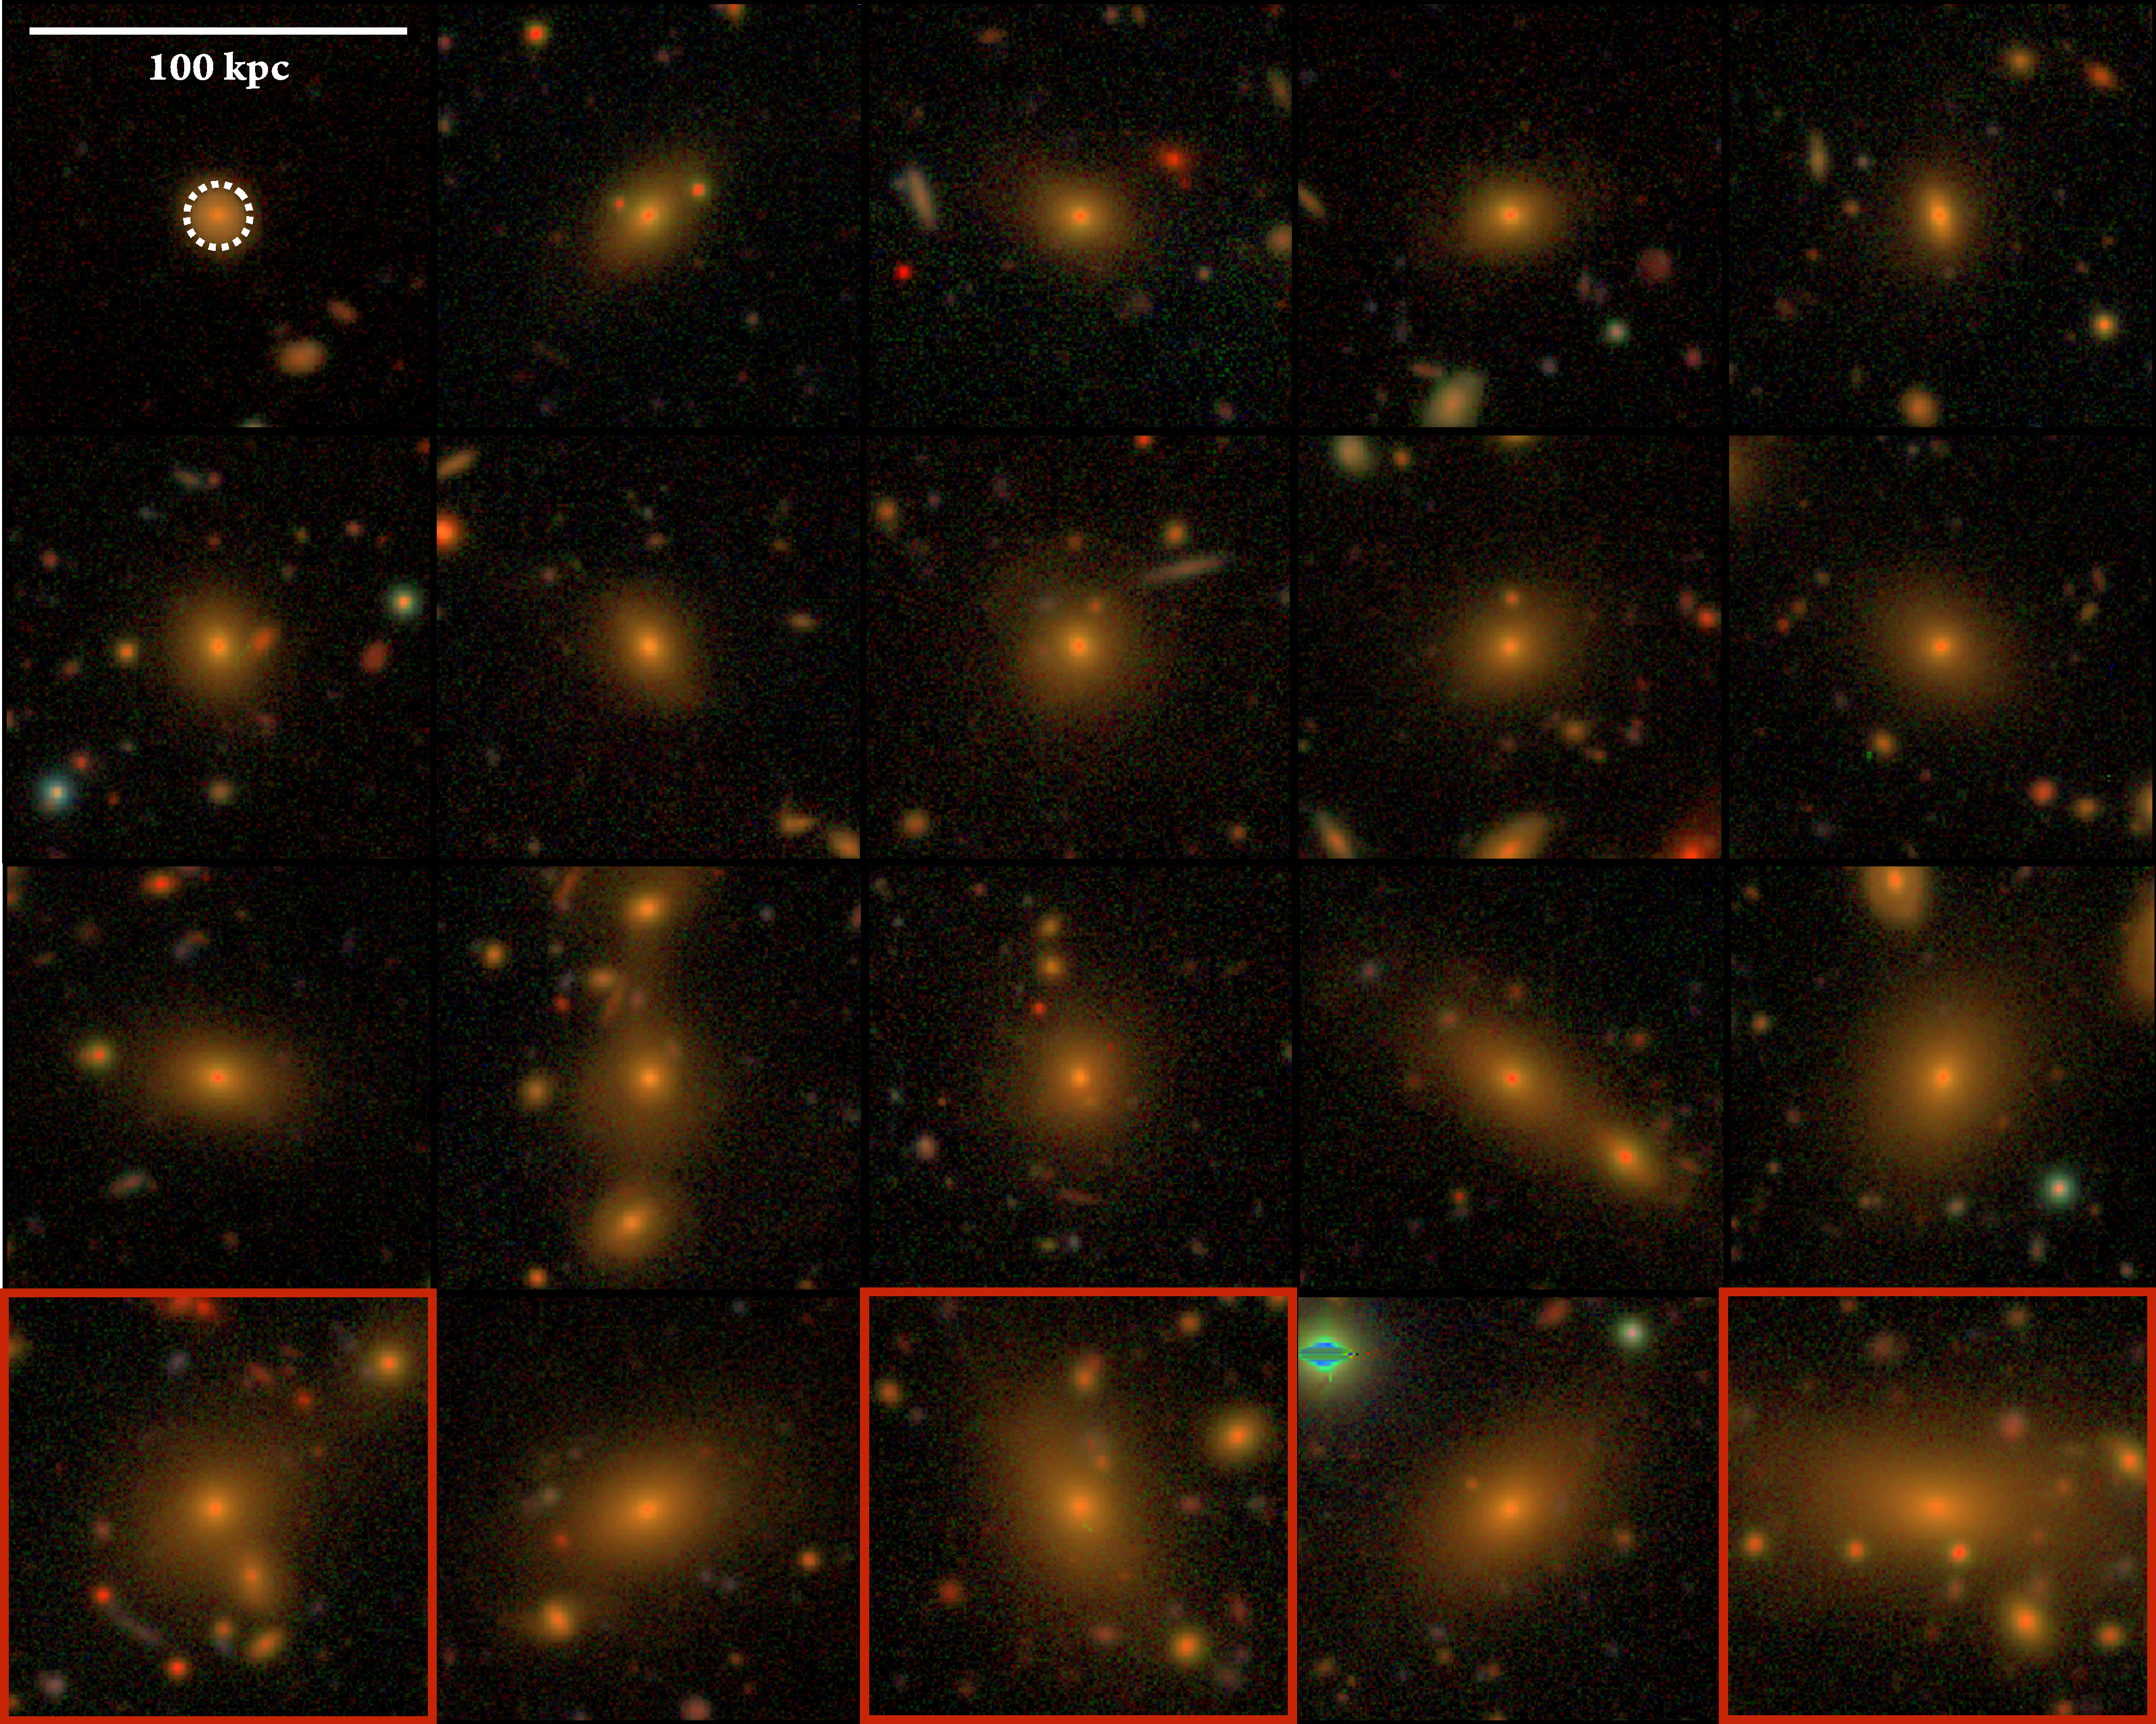
\includegraphics[width=\textwidth]{fig/redbcg_m100_m10_compare}
      \caption{
          Three-colour images for a subsample of massive galaxies at $z{\sim}0.4$. 
          All of these massive galaxies have very similar \mstar{} within a 10-kpc 
          elliptical aperture 
          ($11.2<\log_{10} (M_{\star,10\ \mathrm{kpc}}/M_{\odot})<11.3$). 
          The dashed-line circle at the top-left figure indicates $R=$10 kpc.
          These galaxies are rank-ordered from top to bottom and from left to right 
          by their \mstar{} within a 100-kpc elliptical aperture that varies 
          from $10^{11.2}\ M_{\odot}$ to $10^{11.7}\ M_{\odot}$. 
          At fixed `inner' mass (\minn{}), massive galaxies display significant
          diversity in their outer profiles. 
          Red boxes indicate galaxies from dark matter haloes that are more massive 
          than ${\sim} 10^{14}\ M_{\odot}$. 
          }
      \label{fig:m100_m10_color}
  \end{figure*}
%% ------------------------------------------------------------------------------------ %% 

%% ------------------------------------------------------------------------------------ %% 
  \begin{figure*}
      \centering 
      \includegraphics[width=\textwidth]{fig/redbcg_prof_1}
      \caption{
          The environmental dependence of the stellar mass profiles of massive central 
          galaxies. 
          Left: Halo mass dependence of galaxy profiles at fixed `total' stellar mass 
          (\mtot{}). 
          Right: Halo mass dependence of galaxy profiles at fixed `inner-mass' 
          (\minn{}). Orange and red lines correspond to central galaxies living in 
          haloes with \logmh{} $\geq 14.2$. 
          Black and grey lines correspond to central galaxies living in haloes with 
          \logmh{} $\leq 14.0$. 
          Thin lines show the profiles of individual galaxies, while thick lines show 
          the median profile. 
          The uncertainty on the median profile is given by the shaded region and is 
          computed via bootstrap resampling. 
          Brown lines in the bottom panels show the relative difference between  
          the two median profiles 
          ($\Delta = \log(\mu_{\star, \mathrm{cenHighMh}}) - 
          \log(\mu_{\star, \mathrm{cenLowMh}}$). 
          Errors in the difference between the two profiles are also computed 
          via bootstrap.
          The grey-shaded regions show a Monte Carlo test to assess how likely it is to 
          obtain $\Delta$ from random sub-samples of the data. 
          To compute the grey-shaded regions, we first mix the two samples 
          (\rbcg{} and \nbcg{}), then draw sub-samples of galaxies from the mixed 
          population and compute $\Delta$ in the same fashion as for our fiducial 
          signal. 
          We repeat this process 5000 times.  
          The dark grey--shaded region (light grey--shaded region) shows the 1-$\sigma$ 
          (3-$\sigma$) fluctuations in $\Delta$ from these 5000 draws.
          }
      \label{fig:prof_1} 
  \end{figure*}
%% ------------------------------------------------------------------------------------ %% 

%% ------------------------------------------------------------------------------------ %% 
  \begin{figure*}
      \centering 
      \includegraphics[width=\textwidth]{fig/redbcg_scaling_relation}
      \caption{
          \textbf{Left}: The mass-size relations for \rbcg{} (orange squares) and 
          \nbcg{} (grey dots) galaxies. 
          Two vertical lines highlight our $11.6<$ \logms{} $<11.9$ mass bin. 
          The red solid line shows the best-fitting mass--size relation for \rbcg{} and the 
          grey dashed line shows the best-fitting relation for \nbcg{}. 
          Shaded regions in lighter colours show the 1-$\sigma$ uncertainties
          from Markov chain Monte Carlo (MCMC) sampling.  
          \song{
          The green dashed line shows the mass--size relation for $z<0.09$ central 
          galaxies in massive groups from \citet{HCompany13}. 
          And the cyan dashed line represents the mass--size relation for 
          $0.2<z<0.5$ ETGs in groups from the COSMOS survey provided by 
          \citet{HueartasCompany2013b}.
          }
          \textbf{Right:} The relations between \mtot{} and \minn{} for the 
          \rbcg{} and \nbcg{} galaxies, along with the best-fitting scaling relations for 
          both samples.
          }
      \label{fig:scaling_relation} 
  \end{figure*}
%% ------------------------------------------------------------------------------------ %% 

%% ------------------------------------------------------------------------------------ %% 
%% Sample Selection and Data Reduction
%% ------------------------------------------------------------------------------------ %% 
\section{Sample Selection and Data Reduction}
    \label{sec:data}
    
    We refer the reader to Paper I for an in-depth description of the sample selection 
    and data reduction processes. 
    Here, we briefly summarize the main steps.
    
    We use imaging data from the HSC internal data release 
    \texttt{S15B}, which is very similar to the Public Data Release 1 
    (\citealt{HSC-DR1} and covers ${\sim} 110$ deg$^2$ in all five-band ($grizy$) to 
    the full depth in the wide field. 
    The data are reduced by \texttt{hscPipe 4.0.2}, a derivative of the 
    Large Synoptic Survey Telescope (LSST) pipeline (e.g.\ \citealt{Juric2015}; 
    \citealt{Axelrod2010}), modified for HSC (\citealt{HSC-PIPE}).
    The pixel scale of the reduced image is $0.168$\asec{}.
    We use $i$-band images for extracting surface brightness profiles. 
    HSC $i$-band images are typically 3--4 mag deeper than SDSS 
    (Sloan Digital Sky Survey; e.g., \citealt{SDSS-DR7, SDSS-DR8, SDSS-DR12})  
    and have superb seeing conditions (mean $i$-band seeing has FWHM$=0.6$\asec{}).
    
    In Paper~I, we select a sample of 25286 bright galaxies with spectroscopic 
    redshifts or reliable `red-sequence' photometric redshifts (\citealt{Rykoff2014}) 
    at $0.3<z<0.5$. 
    Within this redshift range, we have a large enough volume 
    ($\sim5\times 10^6$ Mpc$^3$) to sample the galaxy stellar mass function above 
    \logms$>11.6$, and we can spatially resolve galaxies profiles to $\sim 5$ kpc 
    ($1.0^{\arcsec}$ corresponds to 4.4 and 6.1 kpc at $z=0.3$ and 0.5). 
    \song{
    Massive galaxies should experience little structural evolution and 
    size growth between $z=0.5$ and 0.3 ($\sim$1.5 Gyr time span) 
    based on model prediction (e.g., \citealt{Shankar2015}).
    }
    
    After carefully 
    masking out surrounding neighbors and accounting for the subtraction of the 
    background light, we derive $i$-band surface brightness profiles out to 100 kpc. 
    We use the broadband spectral energy distributions (SED) fitting code 
    \texttt{iSEDFit}\footnote{http://www.sos.siena.edu/~jmoustakas/isedfit/} 
    (\citealt{Moustakas13}) to measure \m2l{} ratios and $k$--corrections using 
    five-band forced \cmodel{} magnitudes from \texttt{hscPipe}. 
    We assume a \citet{Chabrier2003} IMF, the Flexible Stellar Population 
    Synthesis models\footnote{http://scholar.harvard.edu/cconroy/sps-models}
    (FSPS; \texttt{v2.4}; \citealt{FSPS}, \citealt{Conroy2010}), the 
    \citet{Calzetti2000} extinction law, and a simple delayed-$\tau$ model for 
    star formation histories (SFH). 
    Using HSC data, we can measure the \mden{} profiles of massive galaxies to 
    $\sim 100$ kpc, and we integrate these profiles within elliptical isophotal
    apertures at different physical radii. 
    As explained in Paper~I, we focus on the two following metric masses:
        
    \begin{itemize}
    
        \item Stellar mass within 10 kpc (hereafter noted \minn{}), which we use 
            as a proxy for the stellar mass of the \textit{in situ} stellar 
            component. 
            This is motivated both by recent observations and simulations 
            (e.g.~\citealt{vanDokkum2010}, \citealt{RodriguezGomez2016}). 
            The value of 10 kpc that we quote here corresponds to the radius of the 
            major axis of the isophotal ellipse.
            
        \item Stellar mass within 100 kpc (hereafter noted \mtot{}). 
            We use \mtot{} as a proxy for the `total' stellar mass. 
            In Paper~I we show that \mtot{} recovers more light compared to 
            HSC \cmodel{} photometry and has offsets that can be a large as 0.2 dex 
            in magnitude.        
               
   \end{itemize}
   
   We use these two simple metric masses to explore the \mstar{}-dependence of the 
   fraction of accreted stars and to reveal the diversity of stellar envelopes among 
   massive galaxies. 
   In practice, we also have the full profiles for each galaxy and can cast our 
   results in terms of the full stellar mass profiles. 
   However, in many cases we find it more useful to display figures using the simpler 
   \minn{} and \mtot{} quantities. 
   In Figure \ref{fig:m100_m10_color}, we highlight the diversity of galaxies as a 
   function of \minn{} and \mtot{}. 
   Figure \ref{fig:m100_m10_color} shows a random subsample of massive galaxies with 
   very similar \minn{} that have a large range of \mtot{}. 
   We use these two aperture masses to guide our comparison of massive galaxies 
   as a function of environment.  
    
%% ------------------------------------------------------------------------------------ %%    
\subsection{Massive Central Galaxies from Different Environments}
    \label{ssec:cen}
         
    In this work, we focus on massive galaxies with \mtot{} $>10^{11.6}$~\msun{}. 
    In Paper~I, we demonstrate that this sample is almost mass complete over our full 
    redshift range. 
    In addition to the mass cut above, we also limit our sample to galaxies that live 
    at the centers of their own dark matter haloes -- so-called `central' galaxies. 
    We use the \redm{} \texttt{v5.10} \citep{Rykoff2014, Rozo2015b} cluster catalogue 
    to help us construct a central galaxy sample.
    
    %Central galaxies are important to the study of galaxy-halo connection and follow 
    %stellar mass--halo mass relation (SHMR; e.g., \citealt{Leauthaud2012, 
    %Behroozi2013, Kravtsov2014, Tinker2017}) at high-\mstar{}.
 
    First, we select 68 massive central galaxies from \redm{} clusters 
    with richness $\lambda \geq 30$, and we assign the probability of true central 
    galaxy $P_{\mathrm{Cen}} \geq 0.7$, and \logmtot{}$ >11.5$ 
    at $0.3 < z < 0.5$ (63/68 have \logmtot{}$ >11.6$). 
    This $\lambda$ limit is chosen to mitigate incompleteness in the cluster catalogue
    at the high end of our redshift window. 
    The $P_{\mathrm{Cen}}$ limit is selected to exclude low-probability candidates for 
    central galaxy. 
    \song{
    \citet{Simet2017} calibrates the \mhalo{}-$\lambda$ relation for the \redm{} 
    clusters using the SDSS weak-lensing data after carefully addressing many 
    important systematic uncertainties.
    Based on this calibration, these clusters correspond to central galaxies living 
    in haloes with \mhalo{}$>10^{14.2}$~\msun{}. 
    This calibration is consistent with several other independent calibrations 
    using different methods (e.g., \citealt{Saro2015, Farahi2016, 
    Melchior2016, Murata2017}). 
    }
    The median richness of the sample is $\lambda \approx 41$ 
    (\mhalo{}$\approx 2.2 \times 10^{14}$~\msun{}), and there are 
    only 44 central galaxies in clusters with $\lambda>50$ 
    (\mhalo{}$\approx 3.0 \times 10^{14}$~\msun{}).
    We refer to this sample of \textbf{central galaxies in massive haloes} as 
    the \rbcg{} sample.
    
    Second, we build a complementary sample of central galaxies in lower mass haloes
    by excluding all galaxies that are in any \redm{} cluster with $\lambda > 20$.
    \song{
    We convert their $\lambda$ into $M_{\mathrm{200b}}$ using calibration by 
    \citet{Simet2017}. Using the \texttt{Colossus} Python package 
    (\citealt{Colossus})\footnote{\url{http://www.benediktdiemer.com/code/colossus/}}
    provided by \citet{Diemer2015}, we estimate the $R_{\mathrm{200b}}$ of each 
    cluster given its $M_{\mathrm{200b}}$ and redshift.
    } 
    We exclude all galaxies within a cylinder around each cluster, with a radius
    equal to $R_{\mathrm{200b}}$ and a length equal to twice the value of the 
    photometric redshift uncertainty of the cluster (typically around 0.015 to 0.025).
    This second sample is dominated by central galaxies living in haloes with
    $M_{\mathrm{200b}} < 10^{14}$~\msun{}; we refer to this sample as \nbcg{}. \
    There are 833 central galaxies with \logmtot{}$> 11.6$ in this sample.

    Satellite contamination should be relative low at the high-\mtot{} end
    (e.g., \citealt{Reid2014, Hoshino2015, Saito2016, vanUitert2016}). 
    For instance, the model from \citet{Saito2016} predicts a $\sim 7$\% 
    fraction for satellite galaxies with \logmtot{}$>11.6$ and \logmh$<14.0$ haloes.
    
    In Appendix~\ref{app:basic}, we show the distributions of redshift, \mtot{}, and 
    \minn{} for the \rbcg{} and \nbcg{} samples. 
    We also compare these two samples on a \mtot{} versus rest--frame $(g-r)$ colour 
    plane. 
    Both of the samples follow the same red-sequence, with only a handful of galaxies 
    displaying bluer colours.
    
    We note that our analysis fails to extract 1-D profiles for $\sim10$\% of 
    \rbcg{} and \nbcg{} galaxies due to ongoing major mergers or projection effects 
    (e.g.\ nearby foreground galaxy or bright stars). 
    However, this small failure rate should not affect any of the results in this paper.
    
%% ------------------------------------------------------------------------------------ %% 

%% ------------------------------------------------------------------------------------ %% 
%% Results 
%% ------------------------------------------------------------------------------------ %% 
\section{Results}
    \label{sec:result}
    
    As shown in Figure~\ref{fig:m100_m10_color}, massive central galaxies at fixed  
    \minn{} display a large diversity in their stellar haloes. 
    In Paper~I, we explore the \mstar{}-dependence of the stellar haloes in massive 
    galaxies, we now investigate the relation between the \mden{} profiles of 
    massive galaxies, their stellar haloes, and dark matter halo mass. 
    %Here we use \mtot{} as a proxy for the `total' \mstar{} of massive galaxies, and 
    %we use \minn{} as a rough proxy for the stellar mass of the \textit{in situ} 
    %component.  
    We remind the reader that although a circular aperture is shown on 
    Fig~\ref{fig:m100_m10_color}, in practice we extract 1-D \mden{} profiles and 
    estimate \mtot{} and \minn{} using elliptical apertures following the average 
    flux-weighted isophotal shape. 

%% ------------------------------------------------------------------------------------ %% 
\subsection{Environmental Dependence of the Stellar Mass Density Profiles of Massive 
            Galaxies}
    \label{ssec:sbp_mtot} 
       
    First, we ask whether the \mden{} profiles of massive central galaxies depend on 
    halo mass at a fixed stellar mass.    
    We show comparisons of \mden{} profiles at both fixed \mtot{} and fixed 
    \minn{}. 
    We also ensure that all comparisons are performed with a fixed underlying redshift
    distribution by matching samples in redshift in addition to a fixed stellar mass
    (please see Appendix~\ref{app:match}, Appendix~\ref{app:redshift}, 
    and Fig~\ref{fig:match} for details). 
   
%% ------------------------------------------------------------------------------------ %%     
    Fig~\ref{fig:prof_1} compares the \mden{} profiles of massive central galaxies 
    living in less massive dark matter haloes (\logmh$<14.0$) to those living in more 
    massive dark matter haloes (\logmh$>14.2$) at fixed \mtot{} (left panel) and at 
    fixed \minn{} (right panel). 
    At fixed \mtot{}, we compare massive galaxies that have similar `total' \mstar{}. 
    On the right side, we use \minn{} as a proxy for the \textit{in situ} \mstar{} to 
    compare the overall \mstar{} distributions of galaxies living in different 
    environments that have assembled a similar amount of stars at high-$z$.
    This figure shows the main result of this paper, namely that 
    \emph{the \mden{} profiles of massive central galaxies show a clear dependence on 
    dark matter halo mass at both fixed \mtot{} and \minn{}.}

    \song{
    We estimate the uncertainties of the median \mden{} profiles using a bootstrap 
    resampling test, and we perform statistical tests to demonstrate that the 
    differences of \mden{} profiles are more significant than the levels allowed by 
    the intrinsic randomness within the combined \rbcg{} and \nbcg{} sample. 
    }
    We also conduct a variety of tests that verify the robustness of these results with
    respect to the choices of \mtot{} bins, $\lambda$ cut, the redshift range, and the 
    choice of apertures used for the metric masses. 
    Please see Appendix~\ref{app:robust} for further details.
    \song{
    In Appendix \ref{app:cog} and Figure~\ref{fig:cog}, we compare the same 
    \mtot{}-matched samples using the cumulative \mstar{} profiles (or `curve of growth') 
    and the fraction of \mtot{} enclosed within different radii.
    Both comparisons highlight the differences in median \mden{} profiles 
    from different angles.   
    }
   
    The key features in Figure~\ref{fig:prof_1} are the following:
    
    \begin{itemize}
        
        \item At fixed \mtot{}, central galaxies in more massive dark matter haloes 
            display shallower \mden{} profiles compared to those from less massive 
            dark matter haloes (i.e., they have flatter inner \mden{} profiles and 
            more significant outer stellar haloes). 
            The median \mden{} profiles of the \rbcg{} and \nbcg{} samples cross 
            each other at ${\sim} 15$-20 kpc, roughly the typical effective radius 
            ($R_{\mathrm{e}}$) of massive galaxies with \logmtot{}$>11.7$--11.8.  
            
        \item \song{
            For the \mtot{}-matched samples, there are some subtle but statistically 
            significant and robust differences between the two median \mden{} profiles.
            Due to the logarithmic scale, the difference in the inner region appears 
            to be very small. 
            Meanwhile, the difference in the \mden{} profile becomes more apparent 
            at $R>50$ kpc scales.  
            }
                                
        \item Massive galaxies with similar \mstar{} within 10 kpc have quite
            different \mtot{} and massive central galaxies in more massive haloes 
            host much more prominent outer stellar haloes. 
    
        \item The similar slopes of the \mden{} profiles within 10 kpc for the 
            \minn{}-matched samples are in sharp contrast with the large 
            \textit{intrinsic} scatter we see in the outer \mden{} profiles. 
            We will discuss the inner \mden{} profiles further in \S~\ref{ssec:cen}
                        
    \end{itemize}

    \song{
    Fig \ref{fig:prof_1} shows that the environmental dependence of the profiles of m
    assive central galaxies is a subtle effect.
    }
    This may explain why previous attempts to detect such dependence using 
    shallower images often failed. In Appendix~\ref{app:robust} (see Fig~\ref{fig:prof_2}) 
    we demonstrate that the environmental signature becomes more prominent for more massive 
    galaxies.
    
    \textbf{In summary, we reliably detect a subtle, but robust halo mass dependence of 
    the profiles of massive central galaxies. 
    This dependence could be driven by the fact that massive halos have a larger minor 
    merger rate compared to less massive haloes. 
    Nondissipative (minor) mergers should not strongly alter the inner \mden{} 
    profiles, but can efficiently build up the outer halo 
    (e.g., \citealt{Hilz2013}, \citealt{Oogi2013})}.
      
%% ------------------------------------------------------------------------------------ %% 

%% ------------------------------------------------------------------------------------ %% 
\subsection{The Environmental Dependence of Scaling Relations}
    \label{ssec:scaling}
    
    We have shown that the \mden{} profiles of massive galaxies 
    show a dependence on the masses of their host dark matter haloes. 
    In this section, we turn our attention to the more commonly studied stellar 
    mass--size relation (\mstar{}--$R_{\mathrm{e}}$). 
    In addition, we consider halo mass dependence on the 
    \mtot{}--\minn{} plane. 
    
%% ------------------------------------------------------------------------------------ %% 
\subsubsection{Mass--Size Relation}
    \label{sssec:mass_size}
    
    The tight relation between \mstar{} and effective radius (or half-light radius; 
    $R_{\mathrm{e}}$ or $R_{\mathrm{50}}$; e.g., \citealt{Shankar2013, Leja2013, 
    vdWel2014}) is one of the most important scaling relationships for ETGs. 
    Despite numerous attempts, previous studies have failed to detect the 
    \mhalo{}-dependence of the \mstar{}--$R_{\mathrm{e}}$ relation at low-$z$ 
    (e.g., \citealt{Weinmann2009, Nair2010, HCompany13, Cerbrian2014}; 
    except for the recent result by \citealt{Yoon2017}). 
    
    \song{
    We emphasize the fact that `size' is not a well-defined parameter for massive 
    galaxies with very extended stellar mass distributions. 
    In practice, the measurements of `effective radius' or `half-light radius' 
    not only depend on resolution, depth, and filter of the image, but may also 
    depend on the adopted model for the light profile.  
    This makes comparisons of size measurements among different observations 
    or between observations and models much more uncertain, and is the main reason
    why we prefer to compare the \mden{} profiles directly.
    }
    In this section, we adopt the radius enclosing 50\% of stellar mass within 
    100 kpc ($R_{\mathrm{50}}$; derived from the $i$-band curve-of-growth) as the 
    `size' for massive galaxies. 
    Such a definition of `half-light radius' is more robust against structural 
    details, choice of model, and the background subtraction compared to the 
    effective radius measured using a 2-D model with oversimplified assumptions 
    (e.g., single-\ser{} model). 
    Massive galaxies in this sample are large enough so that the impact of seeing 
    is not a concern.
    
    The left panel of Fig~\ref{fig:scaling_relation} shows the 
    \mtot{}--$R_{\mathrm{50}}$ relations for galaxies in more and less massive
    dark matter haloes. 
    We fit the \logmtot{}-$\log_{10} (R_{\mathrm{50}}/\mathrm{kpc})$ relations at 
    $\log(M_{\star,100})>11.6$ using the \texttt{emcee} MCMC sampler 
    (\citealt{Emcee})\footnote{The initial guesses are based on maximum 
    likelihood estimates, and we assume flat priors for parameters.}.
    \song{
    Uncertainties in both \mtot{} and $R_{\mathrm{50}}$ are considered. 
    For \logmtot{}$>11.6$ galaxies, the typical uncertainty for mass is $\sim 0.12$
    dex.  
    The $R_{\mathrm{50}}$ uncertainty is based on the \mden{} profile and
    is very small due to the high \s2n{} of the profile. 
    We manually assign a 10\% error for $R_{\mathrm{50}}$. 
    }
    
    The best-fitting relation for \rbcg{} is:
    
    \begin{equation}
        \begin{aligned}
        \log_{10} (R_{\mathrm{50}}/\mathrm{kpc}) = & (0.74\pm0.13) \times \log_{10} (M_{\star, 100\ \mathrm{kpc}}/M_{\odot}) \\ & -(7.56\pm1.56)
        \end{aligned}
    \end{equation}

    \noindent And for \nbcg{}, we find:
    
    \begin{equation}
        \begin{aligned}
        \log_{10} (R_{\mathrm{50}}/\mathrm{kpc}) = & (0.68\pm0.06) \times \log_{10} (M_{\star, 100\ \mathrm{kpc}}/M_{\odot}) \\ & -(6.88\pm0.75)
        \end{aligned}
    \end{equation}
    
    \noindent As shown in the left panel of Fig~\ref{fig:scaling_relation}, 
    massive central galaxies of more and less massive dark matter haloes lie on 
    \mtot{}--$R_{\mathrm{50}}$ relations that have similar slopes but 
    different normalizations. 
    The best-fitting mass--size relation derived here suggests that, 
    at $0.3 < z < 0.5$, central galaxies with \logmtot{}$>11.6$ in \logmhalo{}$>14.2$
    haloes are on average $\sim20$\% larger than the centrals from \logmhalo{}$<14.0$
    haloes at fixed \mtot{}.
    This result is robust against the ranges of \mstar{} over which the fit is 
    performed and against the definitions of  `total' \mstar{} and half-light 
    radius\footnote{Using \mstar{} within 120 or 150 kpc, or using the 
    $R_{\mathrm{50}}$ derived within these apertures do not change the results.}. 
    
    \song{
    Due to the steep slope of the mass--size relation, secondary binning 
    (e.g., different halo mass) may introduce artificial differences 
    (e.g., \citealt{Sonnenfeld2017}).
    Besides the differences in best--fit \mtot{}--$R_{\mathrm{50}}$ relation, the 
    median $R_{\mathrm{50}}$ of the \mtot{}-matched samples also confirm the above 
    conclusion. 
    In addition, we use the normalized size parameter ($\gamma$; e.g., 
    \citealt{Newman2012, HCompany13}) to further test our results. 
    In \citet{HCompany13}, $\gamma$ is defined as:
    }
    
    \begin{equation}
        \log_{10}(\gamma) = \log_{10} (R_{\mathrm{50}}) + \beta (11 - \log_{10}M_{\star, 100\ \mathrm{kpc}}),
    \end{equation}
    
    \song{
    where $\beta$ is the slope of the mass--size relation.
    We estimate the average $\gamma$ of both samples at \logmtot{}$>11.6$. 
    For the \rbcg{} sample, $<\gamma> = 4.2\pm0.4$; for the \nbcg{} one, 
    $<\gamma> = 3.8\pm0.3$. 
    The environmental dependence of $R_{\mathrm{50}}$ at fixed \mtot{} is more 
    significant than the \citet{HCompany13} result, although the uncertainty 
    is large for our small samples. 
    Such environmental dependence of `size' is much weaker than the certain 
    model prediction (e.g., \citealt{Shankar2014}).
    It is important to remember that the uncertainties of both mass and size can 
    wash out signals of stronger environment--dependence on mass--size plane 
    (e.g., \citealt{HCompany13}), and direct comparison of \mden{} profiles or 
    the \mtot{}--\minn{} relation may serve as a better tracer of the environment 
    dependence. 
    }
    
    \song{
    We qualitatively compare our results with the mass--size relation for 
    $0.2 < z < 0.5$ group ETGs in the COSMOS survey (
    \citealt{HueartasCompany2013b}; HC13a; cyan dashed line).
    HC13a measures luminosity and size of each galaxy by fitting a 2--D 
    single--\ser{} model to the \textit{HST}/ACS \texttt{F814W} image. 
    And the stellar mass is derived from SED fitting based on very similar 
    model assumptions. 
    HC13a uses circularized effective radius 
    ($R_{\mathrm{e,Circ}} = R_{\mathrm{e,Fit}} \times \sqrt{b/a}$) in their work. 
    Here we empirically correct their effective radius to the measured values 
    assuming an average $<b/a>=0.75$.
    At similar redshift, the mass-size relation from HC13a lies below our 
    best--fit relation, while the slopes are quite similar.
    }
    
    \song{
    We also compare with results from \citealt{HCompany13} (HC13b; green dashed line), 
    who studied $z\leq 0.09$ central ETGs in $12.5 \le$ \logmh{} $< 15$ haloes. 
    HC13b use the group catalogue by \citet{Yang2007} to estimate halo mass. 
    In contrast to the present study, HC13b find no environment dependence in the 
    mass--size relation for central galaxies in the range $12.5\le$ \logmh{} $<15.0$. 
    They obtain effective radii from single-\ser{} model fitting to SDSS 
    images and \mstar{} based on SED fitting using the BC03 (\citealt{BC03}) 
    synthetic population model. 
    We convert the HC13b \mstar{} estimates from a Kroupa IMF to a Chabrier 
    IMF by applying a constant $-0.05$ dex shift (see \citealt{Bernardi2016a}). 
    We further add $+0.1$dex to the HSC13 stellar masses to account for a systematic 
    offset between BC03 and our FSPS model (see Paper~1). 
    Here we see that our massive galaxies follow the HC13a relation reasonably well
    (with slightly shallower slopes) despite the differences in redshift. 
    }
    
    \song{
    Differences between the HC13ab and our results may relate to differences 
    in modelling methods and the shallower ACS/\texttt{F814W} images. 
    As for HC13b, it is also possible that the shallower SDSS image hides the
    environmental dependence.  
    The low surface--brightness stellar haloes that present the best evidence for 
    environmental dependence using the deep HSC images are impossible to see and 
    are extremely difficult to model using the SDSS ones. 
    Before one can reliably investigate topics such as the environment dependence 
    of mass--size relation and its redshift evolution, impacts from crucial systematics 
    like the imaging qualities and model assumptions much be carefully addressed. 
    Both shallow images and oversimplified models can lead to biased results 
    (e.g., see Appendix~\ref{app:gama} for the issue with single-\ser{} model 
    using SDSS images).
    }

%% ------------------------------------------------------------------------------------ %% 
    
%% ------------------------------------------------------------------------------------ %% 
\subsubsection{\mtot{} - \minn{} Relation}
    \label{sssec:m100_m10}
    
    Now we investigate the relationship between \mtot{}, \minn{}, and \mhalo{}. 
    Compared to the mass--size relation, the \mtot{}--\minn{} relation is not plagued 
    by the ambiguity of galaxy `size', and it also enables a more straightforward 
    comparison with numerical simulations.
    
    The right panel of Fig \ref{fig:scaling_relation} compares \rbcg{} and \nbcg{}
    galaxies on the \mtot{}--\minn{} plane. 
    We find that there is an offset between the overall distributions of these two
    samples and that they follow distinct best-fitting \mtot{}--\minn{} relations. 
    For \rbcg{} galaxies with \logmtot{}$>11.6$ we find:
    
    \begin{equation}
        \begin{aligned}
        \log_{10} (M_{\star, 10\ \mathrm{kpc}}/M_{\odot}) = & (0.48\pm0.06) \times \log_{10} (M_{\star, 100\ \mathrm{kpc}}/M_{\odot}) \\ & +(5.72\pm0.75).
        \end{aligned}
    \end{equation}
    
    \noindent In the same range of \mtot{}, the best-fitting relation for \nbcg{} is:
     
    \begin{equation}
        \begin{aligned}
        \log_{10} (M_{\star, 10\ \mathrm{kpc}}/M_{\odot}) = & (0.56\pm0.03) \times \log_{10} (M_{\star, 100\ \mathrm{kpc}}/M_{\odot}) \\ & +(4.82\pm0.30).
        \end{aligned}
    \end{equation}
    
    These results are robust against the exact choice for the \mtot{} range over which 
    the fit is performed. 
    These results are also robust when we replace \minn{} with the stellar 
    mass within a 5- or 15-kpc aperture, or if \mtot{} is replaced with a stellar mass 
    within a 120- or 150-kpc aperture.  
    
    \song{
    From Figure \ref{fig:scaling_relation} we can draw the same conclusions as in 
    the previous section, namely that at fixed \mtot{}, central galaxies in more massive 
    haloes tend to have a smaller fraction of stellar mass in their inner regions and 
    higher \mstar{} in their outer stellar haloes.  
    }
    
    
    %Meanwhile, at fixed \minn{} -- a proxy for the \mstar{} of the `\textit{in situ}' 
    %component -- central galaxies in more massive haloes tend to be more massive and 
    %display more prominent stellar haloes. 
    %\song{
    %The comparison of \mden{} profiles for \minn{}-matched samples may not directly
    %reflect the environment-related processes because other physical mechanisms could 
    %also change the inner \mden{} profiles and their \mtot{} could be quite different. 
    %But the combination of \mtot{} and \minn{} clearly suggests that information about
    %their dark matter haloes or environments is encoded within this simple 2-D plane. 
    %We discuss more scientific implications of these results in 
    %\S~\ref{sec:discussion}
    %}
     
%% ------------------------------------------------------------------------------------ %% 

%% ------------------------------------------------------------------------------------ %% 
  \begin{figure*}
      \centering 
      \includegraphics[width=\textwidth]{fig/redbcg_ell_color_environ}
      \caption{
          Radial variations in ellipticity and optical colours for massive galaxies. 
          The format of this figure is similar to the right hand side of 
          Fig~\ref{fig:prof_1}. 
          Top panels show the ellipticity profile, middle panels show $g-r$, and lower 
          panels show $g-i$. 
          We compare our results with those from \citet{Tal2011}
          (solid blue line on top panels). 
          We also compare our results with those from a stacking analysis of nearby 
          massive galaxies with high concentration indices ($C>2.6$) from 
          \citet{DSouza2014} (blue dashed lines in top and middle panels). 
          We also compare our results with the average $g-r$ and $g-i$ colour profiles 
          from a large sample of nearby elliptical galaxies for \citet{LaBarbera2010}
          (blue, solid lines in middle and bottom panels).
          }
      \label{fig:ell_color}
  \end{figure*}
%% ------------------------------------------------------------------------------------ %% 


%% ------------------------------------------------------------------------------------ %% 
\subsection{Ellipticity and Colour Profiles}
    \label{ssec:ell_color}
    
    In Paper~I, we show that the ellipticity of the outer stellar halo increases with
    \mtot{}, while in contrast, rest-frame colour gradients do not display strong 
    \mtot{} dependencies. 
    In this paper, we take this analysis one step further to investigate whether either 
    of these quantities display a halo mass dependency. 
    We focus on ellipticity and colour profiles within 5--60 kpc where we can ignore
    differences in sky subtraction and seeing across different filters. 
    Galactic extinction and $k$ corrections are applied to both $(g-r)$ and $(g-i)$ 
    colour profiles.
    
    Figure \ref{fig:ell_color} shows the average ellipticity, $g-r$, and $g-i$ colour 
    profiles for galaxies living in more and less massive dark matter haloes at both 
    fixed \mtot{} and fixed \minn{}. 
    We also compared our results with previous studies that are based on stacked SDSS 
    images (e.g., \citealt{LaBarbera2010, Tal2011, DSouza2014}). 
    Figure \ref{fig:ell_color} shows that: 
    
    \begin{itemize}
        \item \song{
            The ellipticity profiles of massive central galaxies do not depend on 
            halo mass at fixed \mtot{} at $R<60$ kpc. 
            }       
                
        \item \song{
            However, the ellipticities of massive galaxies are different in the 
            outskirts at fixed \minn{}. 
            This further suggests that the more elongated outer stellar haloes 
            of massive haloes may relate to accreted stars.
            }
                     
        \item Massive central galaxies in more and less massive dark matter haloes 
            display similar rest-frame colour gradients (at $r<60$ kpc) at fixed 
            \mtot{} and at fixed \minn{}.    
            
    \end{itemize}
    
    The fact that we find smooth ellipticity profiles and shallow gradients favors 
    the idea of using the flux-weighted average isophotal shape to extract 1-D \mden{} 
    profiles of massive galaxies. 
    The similarity of average rest-frame colour profiles between the \rbcg{} and \nbcg{}
    samples suggests that \mden{} profiles based on single average \m2l{} will not bias 
    our comparisons. 
    
    \song{
    Our work does not address color gradients below 5--6 kpc because we do not deconvolve 
    for the PSF. 
    Color gradients on these scales may be sensitive to other physical processes and 
    deserve future investigation using a 2-D modelling method and/or images with higher 
    spatial resolution.
    }
    
%% ------------------------------------------------------------------------------------ %%    
   
%% ------------------------------------------------------------------------------------ %% 
%% Discussion 
%% ------------------------------------------------------------------------------------ %% 

%% ------------------------------------------------------------------------------------ %% 
\section{Discussion}
    \label{sec:discussion}

%% ------------------------------------------------------------------------------------ %% 
\subsection{The Role of Environment in the Two-Phase Formation Scenario}
            
    Using deep images from the HSC survey, we show that the stellar mass distributions 
    of massive central galaxies at $0.3 < z < 0.5$ depend on their environment or 
    \mhalo{}. 
    At fixed \mtot{} or \minn{}, we find that central galaxies from more massive 
    haloes on average have a larger half-light radius and host more prominent outer 
    stellar haloes. 
    
    \song{
    The two-phase formation scenario can qualitatively explain these results. 
    In this scenario, intense dissipative processes at $z > 2$ are responsible for the 
    formation of \textit{in situ} stars in massive central galaxies. 
    After the rapid quenching of star formation, the assembly of massive galaxies in 
    the second phase is dominated by accretion of satellite galaxies through (mostly) 
    non--dissipative mergers. 
    Dry minor mergers are efficient at depositing \textit{ex situ} stars in the 
    outskirts of massive galaxies (e.g., \citealt{Oogi2013, Bedorf2013}). 
    If minor mergers become more frequent in more massive dark matter haloes, 
    they can result in slightly different stellar mass distributions and larger 
    effective radii for massive central galaxies.
    }
      
    \citet{Shankar2014} studied the environment dependence of galaxy size using 
    different semi-analytic models. 
    They predict that at fixed stellar mass, the median size of central galaxies 
    should increase strongly with halo mass. 
    \song{
    Although the major-merger rate does not strongly depend on halo mass 
    (mass ratio $>1$:3; e.g., \citealt{Hirschmann2013, Shankar2015}), the 
    minor--merger rate could still increase with halo mass if the dynamical friction
    time is short (e.g., \citealt{Newman2012}). 
    Therefore, massive central galaxies with $11.5 <$\logms{}$<12.0$ from 
    massive haloes (\logmh{}$>14.0$) can have up to four times more minor mergers 
    (1:100--1:3) compared to those in less massive haloes at a similar stellar 
    mass. 
    An increase in the minor-merger rate as a function of halo mass can lead to a 
    halo-mass dependence in the mass--size relation. 
    }
    The predictions from \citet{Shankar2014} have been confirmed by \citet{Yoon2017} 
    using the semi-analytic model from \citet{Guo2011}.  
    
    \song{
    Our results are broadly consistent with these predictions and also suggest that 
    the outer stellar haloes ($r>50$ kpc) of massive galaxies show the strongest 
    variations with halo mass. 
    At the same time, we should point out that the comparison at low redshift alone 
    cannot rule out some other scenarios.  
    For instance, \citet{Buchan2016} suggest that central galaxies in more massive 
    haloes could be born with more extended structure. 
    A more careful comparison with higher redshift observations can distinguish between 
    these different scenarios.
    }
   
%% ------------------------------------------------------------------------------------ %% 
\subsection{Environmental Dependence of the Inner Regions of Massive Galaxies}

    Our results also show that the centrals of more massive haloes have slightly 
    shallower inner \mden{} slopes and a smaller \mtot{} fraction within the inner 
    10 kpc.
    \song{
    This cannot be solely explained by the choice of a finite aperture to 
    estimate `total' \mstar{}: Assuming that centrals from more massive haloes 
    have more extended \mden{} profiles, integration out to a larger aperture makes 
    the differences between \rbcg{} and \nbcg{} galaxies on the \mtot{}--\minn{} 
    plane even more significant.
    However, from this observation alone, we cannot determine which exact physical 
    process is responsible for differences in the inner regions. 
    Many different physical processes can shape and alter the \mden{} profile within 
    the inner 10 kpc.
    } 
    
    \song{
    In hydrodynamic simulations, intense dissipative processes help create a 
    self-similar de~Vaucouleurs--like ($n{\sim} 4$) \mden{} profile in the inner
    part of massive galaxy (e.g., \citealt{Hopkins2008}).
    } 
    Major mergers can redistribute the inner stellar mass distributions, but 
    the major--merger rate does not strongly depend on halo mass 
    (e.g., \citealt{Shankar2014}). 
    However, minor mergers, which do depend on halo mass, can modify the central 
    surface brightness profiles of the remnants (e.g., \citealt{BoylanKolchin2007}). 
    Depending on the structure and infalling orbits of satellites, a minor merger 
    can make the inner \mden{} profiles either steeper or shallower.  
    Interestingly, \citet{BoylanKolchin2007} find that when a satellite is accreted 
    from a highly eccentric and energetic orbit to a core--elliptical galaxy, the 
    process tends to reduce the central \mden{}.  
    This is relevant here, as many massive ETGs are known to be core--elliptical 
    galaxies. 
    
    \song{
    Strong adiabatic expansion induced by powerful AGN feedback is another mechanism 
    (e.g., \citealt{Fan2008}) that can modify the inner \mden{} profile. \
    When the induced mass loss is efficient enough, it can lead to expanded 
    central stellar mass distribution and can significantly lower the inner \mden{}. 
    } 
    
    Finally, the coalescence of super-massive black holes (SMBHs) can also flatten 
    the central \mden{} profile via an efficient scattering effect 
    (e.g., \citealt{Milosavljevi2002}).
    On the right side of Fig \ref{fig:scaling_relation}, there are a few candidates 
    for galaxies with large cores. 
    These may be similar to the recently discovered massive brightest cluster galaxies 
    (BCGs) with very large depleted cores (a few thousand parsecs; e.g., 
    \citealt{Postman2012, LopezCruz2014, Thomas2016, Bonfini2016}) possibly resulting 
    from SMBH mergers.
    
    \song{
    The impact of these processes on the \mden{} profiles and their dependency on 
    \mhalo{} are important issues that deserve more investigations. 
    We plan to shed further light on the very inner regions of these massive galaxies 
    using higher resolution images and 2-D modelling to account for the PSF.
    }

%% ------------------------------------------------------------------------------------ %% 

%% ------------------------------------------------------------------------------------ %% 
\subsection{Comparison with Previous Work} 

    Many previous works that focused on the mass--size relation found this relation 
    to be independent of halo mass or environment at $z\sim 0.0$ 
    (e.g., \citealt{Nair2010, Maltby2010, Cappellari2013, HCompany13}). 
    We argue that, both the shallower imaging depth and the oversimple model 
    (e.g., single-\ser{} or de~Vaucouleurs model) used in the fitting can both 
    contribute to this difference.
    In Appendix~\ref{app:gama}, we use the \rbcg{} and \nbcg{} galaxies that overlap 
    with the Galaxy And Mass Assembly (GAMA) survey to demonstrate this point. 
    We show that, for galaxies with similar \mstar{} derived from single-\ser{} 
    models using shallower SDSS images (\citealt{Kelvin2012}), the ones in more 
    massive dark matter haloes actually show more prominent outer stellar haloes.
    \song{
    These issues complicate the comparisons of mass--size relations derived from 
    different images or using different methods.
    }
    
    At low redshift, \citet{Cerbrian2014} find that ETGs with \logms{}$>11.5$ are 
    slightly larger in more massive haloes, and they also show that this trend is 
    reversed at lower \mstar{}. 
    \song{
    \citet{Kuchner2017} use one massive cluster at $z=0.44$ to show that ETGs in 
    that cluster have larger sizes than ETGs in the `field'. 
    }
    \citet{Yoon2017} present a careful study of a large sample of $z\sim0.1$ SDSS 
    ETGs using a nonparametric method; in their research, they recover a clear 
    environment dependence of mass--size relation at \logms{}$>11.2$. 
    They conclude that, at the same \mstar{}, massive ETGs from dense environment 
    are 20--40\% larger compared to those in an underdense environment.
    Recently, \citet{Charlton2017} use a single-\ser{} model for galaxies at 
    $0.2 < z < 0.8$ in the Canada France Hawaii Lensing Survey (CFHTLenS) 
    (\citealt{Heymans2012}) and their galaxy--galaxy 
    lensing measurements to show that larger galaxies tend to live in more massive 
    dark matter haloes (also see \citealt{Sonnenfeld2017}).
    These results are in broad agreement with those presented here.
    \song{
    With the help of weak lensing measurements using HSC images, we will in future 
    work further explore the connection between the dark matter halo mass and the 
    stellar mass distributions of their central galaxies. 
    }
    
    \song{
    As it becomes clear that structures of massive galaxies do depend on 
    environment, the origin of such dependence and its redshift evolution 
    naturally becomes the focus of future studies. 
    Several works find strong environment dependence of the mass--size relation 
    for massive quiescent or early-type galaxies
    (e.g., \citealt{Papovich2012, Bassett2013, Lani2013, Strazzullo2013, 
    Delaye2014}), while other observations suggest otherwise (e.g., 
    \citealt{Rettura2010, Raichoor2012, Kelkar2015, Allen2015}). 
    Comparison with high--redshift results are complicated by many issues and 
    is beyond the scope of this work, but we want to emphasize again that 
    direct comparison of \mden{} profile (e.g., \citealt{Szomoru2012, Patel2013, 
    Buitrago2017, Hill2017}) could better trace the redshift evolution of the
    environment dependence. 
    }
    
    %\song{
    %It is interesting to see that several of these works report stronger 
    %environment dependence of size at fixed \mstar{} for either ETGs or quiescent 
    %galaxies (30--50\% larger in denser environments).
    %As shown in \citet{HCompany13} using a Monte Carlo test (see their \S~4.2), 
    %when the uncertainties of mass and size are considered, the size difference at 
    %fixed stellar mass could be even more significant between extremely different
    %environments.
    %If true, it indicates that denser regions at high redshift ($z>2$) could accelerate 
    %galaxy evolution (e.g., proto-clusters; see \citealt{Wang2016, Shimakawa2018}), and 
    %the size evolution of massive galaxies in a richer environment gradually slows down
    %toward lower redshift (e.g., \citealt{Papovich2012, Andreon2016}.
    %}
    %However, there are also observations that suggest otherwise (e.g., 
    %\citealt{Rettura2010, Raichoor2012, Kelkar2015, Allen2015}). 
    %\song{
    %Comparisons of our results with work done at high redshift are complicated by many 
    %issues. 
    %At high-$z$, these works often rely on small samples or special environments 
    %(rare massive proto-clusters). 
    %Progenitors of massive galaxies in this work may still be star-forming or 
    %late-type galaxies at $z>1$. 
    %Finally, it is just intrinsically more difficult to accurately measure 
    %\mstar{} and size at high redshift (e.g., \citealt{Price2017}).
    %It would be interesting to see whether the current simulations can reproduce 
    %these observed environment dependencies and use them to investigate the redshift
    %evolution of such dependence. 
    %Meanwhile, direct comparisons of rest-frame surface brightness or \mden{} 
    %profiles (e.g., \citealt{Szomoru2012, Patel2013, Buitrago2017, Hill2017}) could be 
    %a better approach than the 
    %mass--size relation to compare high- and low-$z$ mass galaxies.
    %}
    
%% ------------------------------------------------------------------------------------ %% 
\subsection{Towards Consistent Size Definitions}
        
    Until recently, semi-analytic models and hydrodynamic simulations have had
    difficulty reproducing the mass--size relation of massive galaxies. 
    Galaxy sizes are sensitive to many different physical processes (star-formation, 
    feedback, mergers), and matching the galaxy stellar-mass function does not 
    automatically guarantee a match to the mass--size relation. 
    Furthermore, while some efforts have been made to use consistent size definitions 
    (\citealt{McCarthy2017}), more often than not, comparisons of the mass--size relation 
    do not use consistent size definitions, or they only perform crude size conversions 
    (e.g., 3-D radii in simulation versus 2-D projected radii in observation; 
    \citealt{Genel2017}). 
    Observers often quote `sizes' corresponding to the half-light radius along the 
    major axis using 2-D projected images. 
    Simulations, on the other hand, often employ sizes that correspond to the 3-D 
    aperture half-mass radius (e.g., \citealt{Price2017}). 
    
    As emphasized earlier, definitions of galaxy `size' in observations are also not 
    always consistent. 
    Measurements of `size' depend on image quality (e.g., seeing, imaging depth), filter, 
    and the adopted method. 
    Although the elliptical single-\ser{} model is widely adopted in measuring the 
    size of galaxies of different types and at different redshifts, it sometimes leads
    to biased results as it is no longer an appropriate model for certain types of galaxies. 
    Sizes derived from a 1-D curve-of-growth is more model independent and has been 
    shown to be useful in revealing environmental dependence of the mass--size relation 
    (e.g., \citealt{Yoon2017}, and this work), but it does not take the PSF convolution 
    effect into account, and it depends on imaging depth and background subtraction.

    In this paper, we quote stellar masses measured within elliptical apertures of 
    fixed physical size. 
    We argue that this approach will allow for a more straightforward comparison 
    between observations and theoretical predictions.  
          
%% ------------------------------------------------------------------------------------ %% 

%% ------------------------------------------------------------------------------------ %% 
%% Summary 
%% ------------------------------------------------------------------------------------ %% 

%% ------------------------------------------------------------------------------------ %% 
\section{Summary and Conclusions}
    \label{sec:summary}
    
    Using high-quality images from the first $\sim100$ deg$^2$ of the 
    Hyper Suprime-Cam Subaru Strategic Program, we group a large sample of massive 
    central galaxies at $0.3 < z < 0.5$ into two categories based on their dark matter
    halo mass (\mhalo{}$\simgt 10^{14.2} M_{\odot}$ and 
    \mhalo{}$\simlt 10^{14} M_{\odot}$), and we study how their stellar mass 
    distributions out to 100 kpc depend on their environments (or \mhalo{}). 
    Our main results are as follows:  
    
    \begin{enumerate}
    
        \item At fixed \mtot{}, we find that massive central galaxies display \mden{} 
            profiles that have large intrinsic scatter in the outer stellar haloes and 
            present a subtle but systematic trend with \mhalo{}.
            On average, massive central galaxies in more massive haloes have slightly 
            shallower inner \mden{} profiles and more prominent outer haloes. 
            This suggests that the environment affects the assembly of massive central
            galaxies at fixed `total' stellar mass.
            
        \item At fixed \minn{}, massive central galaxies in more massive haloes 
            possess much more extended stellar haloes than those in smaller haloes. 
            Assuming that \minn{} traces the amount of `\textit{in situ}' stars in 
            massive galaxies, this result is consistent with the picture that more 
            massive haloes favor the growth of extended stellar haloes in their central 
            galaxies through more frequent mergers. 
        
        \item \song{
            Such environmental dependence is also reflected on the plane of
            \mtot{} versus $R_{\mathrm{50}}$, and \mtot{} versus \minn{}. 
            And we propose that the \mtot{}-\minn{} relation can be a better tool 
            to diagnose the assembly of massive central galaxies without using `size' 
            with ambiguous definition.
            }
                    
        \item \song{
            At $R < 60$ kpc, the ellipticity and rest--frame colour profiles of 
            massive galaxies do not depend on halo mass at fixed \mtot{}.
            And, at fixed \minn{}, massive centrals from more massive haloes tend 
            to have more elongated outer stellar envelopes.
            } 
             
    \end{enumerate}
    
    These results highlight the importance of deep, high-quality images for studying 
    the assembly of massive haloes and their central galaxies. 
    We are currently working on combining the current results with weak lensing 
    measurements of dark matter haloes around these massive galaxies, and comparing 
    our results with hydrodynamic simulations to gain more physical insight. 

%% ------------------------------------------------------------------------------------ %% 

%% ------------------------------------------------------------------------------------ %% 
%% Acknowledgements 
%% ------------------------------------------------------------------------------------ %% 
\section*{Acknowledgements}

  % Personal 
  The authors thank Frank van~den~Bosch for insightful discussions and 
  Shun Saito for helping us estimate the fraction of satellite galaxies in our sample.
  SH thanks Feng-Shan Liu for sharing the \mden{} profile of the $z\sim1$ BCG from 
  his work.

  % HSC part
  The Hyper Suprime-Cam (HSC) collaboration includes the astronomical communities of 
  Japan and Taiwan, and Princeton University.  The HSC instrumentation and software were
  developed by National Astronomical Observatory of Japan (NAOJ), Kavli Institute
  for the Physics and Mathematics of the Universe (Kavli IPMU), University of Tokyo,
  High Energy Accelerator Research Organization (KEK), Academia Sinica Institute
  for Astronomy and Astrophysics in Taiwan (ASIAA), and Princeton University.  
  Funding was contributed by the FIRST program from Japanese Cabinet Office,  Ministry 
  of Education, Culture, Sports, Science and Technology (MEXT), Japan Society for 
  the Promotion of Science (JSPS), Japan Science and Technology Agency (JST), Toray 
  Science Foundation, NAOJ, Kavli IPMU, KEK, ASIAA, and Princeton University.
   
  % SDSS part
  Funding for SDSS-III has been provided by Alfred P. Sloan Foundation, the 
  Participating Institutions, National Science Foundation, and U.S. Department of
  Energy. The SDSS-III website is http://www.sdss3.org.  SDSS-III is managed by the
  Astrophysical Research Consortium for the Participating Institutions of the SDSS-III
  Collaboration, including University of Arizona, the Brazilian Participation Group,
  Brookhaven National Laboratory, University of Cambridge, University of Florida, the
  French Participation Group, the German Participation Group, Instituto de Astrofisica
  de Canarias, the Michigan State/Notre Dame/JINA Participation Group, Johns Hopkins
  University, Lawrence Berkeley National Laboratory, Max Planck Institute for
  Astrophysics, New Mexico State University, New York University, Ohio State University,
  Pennsylvania State University, University of Portsmouth, Princeton University, the
  Spanish Participation Group, University of Tokyo, University of Utah, Vanderbilt
  University, University of Virginia, University of Washington, and Yale University.
  
  % Pan-STARRS1 part
  The Pan-STARRS1 surveys (PS1) have been made possible through contributions of  
  Institute for Astronomy; University of Hawaii; the Pan-STARRS Project Office; 
  the Max-Planck Society and its participating institutes: the Max Planck Institute 
  for Astronomy, Heidelberg, and the Max Planck Institute for Extraterrestrial Physics, 
  Garching; Johns Hopkins University; Durham University; University of Edinburgh; 
  Queen's University Belfast; Harvard-Smithsonian Center for Astrophysics; Las 
  Cumbres Observatory Global Telescope Network Incorporated; National Central 
  University of Taiwan; Space Telescope Science Institute; National Aeronautics 
  and Space Administration under Grant No. NNX08AR22G issued through the Planetary 
  Science Division of the NASA Science Mission Directorate; National Science 
  Foundation under Grant No. AST-1238877; University of Maryland, and Eotvos 
  Lorand University. 
  
  % LSST software
  This paper makes use of software developed for the Large Synoptic Survey 
  Telescope. We thank the LSST project for making their code available as free 
  software at http://dm.lsstcorp.org.
 
  % KITP
  This research was supported in part by National Science Foundation under Grant 
  No. NSF PHY11-25915. 
  
  % Software
  This research made use of:
  \href{http://www.stsci.edu/institute/software_hardware/pyraf/stsci\_python}{\texttt{STSCI\_PYTHON}},
      a general astronomical data analysis infrastructure in Python. 
      \texttt{STSCI\_PYTHON} is a product of the Space Telescope Science Institute, 
      which is operated by Association of Universities for Research 
      in Astronomy (AURA) for NASA;
  \href{http://www.scipy.org/}{\texttt{SciPy}},
      an open source scientific tool for Python (\citealt{SciPy});
  \href{http://www.numpy.org/}{\texttt{NumPy}}, 
      a fundamental package for scientific computing with Python (\citealt{NumPy});
  \href{http://matplotlib.org/}{\texttt{Matplotlib}}, 
      a 2-D plotting library for Python (\citealt{Matplotlib});
  \href{http://www.astropy.org/}{\texttt{Astropy}}, a community-developed 
      core Python package for astronomy (\citealt{AstroPy}); 
  \href{http://scikit-learn.org/stable/index.html}{\texttt{scikit-learn}},
      a machine-learning library in Python (\citealt{scikit-learn}); 
  \href{http://www.astroml.org/}{\texttt{astroML}}, 
      a machine-learning library for astrophysics (\citealt{astroML});
  \href{https://ipython.org}{\texttt{IPython}}, 
      an interactive computing system for Python (\citealt{IPython});
  \href{https://github.com/kbarbary/sep}{\texttt{sep}} 
      Source Extraction and Photometry in Python (\citealt{PythonSEP});
  \href{https://jiffyclub.github.io/palettable/}{\texttt{palettable}},
      colour palettes for Python;
  \href{http://dan.iel.fm/emcee/current/}{\texttt{emcee}}, 
      Seriously Kick-Ass MCMC in Python;
  \href{http://bdiemer.bitbucket.org/}{\texttt{Colossus}}, 
      COsmology, haLO and large-Scale StrUcture toolS (\citealt{Colossus}).

%% ------------------------------------------------------------------------------------ %% 
%% References  
%% ------------------------------------------------------------------------------------ %% 
\bibliographystyle{mnras}
\bibliography{redbcg}

%% ------------------------------------------------------------------------------------ %% 
%% Table.1 
%% ------------------------------------------------------------------------------------ %% 
\clearpage
\begin{deluxetable}{c ccc ccc}[b!]
\tabletypesize{\scriptsize}
\tablewidth{0pt}
\tablecolumns{7}
\tablenum{1}
\tablecaption{Median \mden{} Profiles of Massive Galaxies in Different Stellar Mass Bins}
%% ------------------------------------------------------------------------------------ %% 
\tablehead{
    \colhead{$R/\mathrm{kpc}$} & 
    \multicolumn{3}{c}{\mden{} ($\log (M_{\odot}/\mathrm{kpc}^2)$) for \rbcg{}} &
    \multicolumn{3}{c}{\mden{} ($\log (M_{\odot}/\mathrm{kpc}^2)$) for \nbcg{}}
	\vspace{1.4ex}
    %------------------------------------------------------------------------------------%
    \nl 
    \colhead{} & 
    \colhead{$\log \frac{M_{\star,100\mathrm{kpc}}}{M_{\odot}}\in$[11.5, 11.7]} & 
    \colhead{[11.7, 11.9]} & 
    \colhead{[11.9, 12.2]}\hspace{2.0ex} & 
    \colhead{[11.2, 11.5]} & 
    \colhead{[11.5, 11.7]} & 
    \colhead{[11.7, 11.9]}
    %------------------------------------------------------------------------------------%
	\vspace{1.6ex}
    %------------------------------------------------------------------------------------%
    \nl
    \colhead{    (1)} &
    \colhead{    (2)} &
    \colhead{    (3)} &
    \colhead{    (4)} &
    \colhead{    (5)} &
    \colhead{    (6)} &
    \colhead{    (7)}
    %------------------------------------------------------------------------------------%
}
%% ------------------------------------------------------------------------------------ %% 
\startdata
%% ------------------------------------------------------------------------------------ %% 

 0.0 & $ 9.30\substack{+0.02 \\ -0.02}$ &$ 9.33\substack{+0.02 \\ -0.02}$ &$ 9.34\substack{+0.02 \\ -0.03}$ &$ 9.36\substack{+0.00 \\ -0.00}$ &$ 9.27\substack{+0.00 \\ -0.00}$ &$ 9.32\substack{+0.01 \\ -0.01}$ \\
 0.5 & $ 9.28\substack{+0.02 \\ -0.02}$ &$ 9.31\substack{+0.02 \\ -0.02}$ &$ 9.32\substack{+0.03 \\ -0.02}$ &$ 9.33\substack{+0.00 \\ -0.00}$ &$ 9.25\substack{+0.00 \\ -0.00}$ &$ 9.30\substack{+0.01 \\ -0.01}$ \\
 0.8 & $ 9.25\substack{+0.02 \\ -0.02}$ &$ 9.28\substack{+0.02 \\ -0.02}$ &$ 9.30\substack{+0.02 \\ -0.02}$ &$ 9.29\substack{+0.00 \\ -0.00}$ &$ 9.22\substack{+0.00 \\ -0.00}$ &$ 9.27\substack{+0.01 \\ -0.01}$ \\
 1.2 & $ 9.22\substack{+0.02 \\ -0.02}$ &$ 9.25\substack{+0.02 \\ -0.02}$ &$ 9.28\substack{+0.02 \\ -0.02}$ &$ 9.24\substack{+0.00 \\ -0.00}$ &$ 9.19\substack{+0.00 \\ -0.00}$ &$ 9.24\substack{+0.01 \\ -0.01}$ \\
 1.5 & $ 9.16\substack{+0.02 \\ -0.01}$ &$ 9.20\substack{+0.02 \\ -0.02}$ &$ 9.24\substack{+0.02 \\ -0.02}$ &$ 9.17\substack{+0.00 \\ -0.00}$ &$ 9.14\substack{+0.00 \\ -0.00}$ &$ 9.20\substack{+0.01 \\ -0.01}$ \\
 1.9 & $ 9.10\substack{+0.01 \\ -0.01}$ &$ 9.14\substack{+0.02 \\ -0.01}$ &$ 9.19\substack{+0.02 \\ -0.02}$ &$ 9.08\substack{+0.00 \\ -0.00}$ &$ 9.08\substack{+0.00 \\ -0.00}$ &$ 9.15\substack{+0.01 \\ -0.01}$ \\
 2.2 & $ 9.03\substack{+0.01 \\ -0.01}$ &$ 9.08\substack{+0.01 \\ -0.01}$ &$ 9.14\substack{+0.02 \\ -0.02}$ &$ 9.00\substack{+0.00 \\ -0.00}$ &$ 9.01\substack{+0.00 \\ -0.00}$ &$ 9.09\substack{+0.01 \\ -0.01}$ \\
 2.5 & $ 8.97\substack{+0.01 \\ -0.01}$ &$ 9.03\substack{+0.01 \\ -0.01}$ &$ 9.10\substack{+0.02 \\ -0.02}$ &$ 8.93\substack{+0.00 \\ -0.00}$ &$ 8.96\substack{+0.00 \\ -0.00}$ &$ 9.04\substack{+0.01 \\ -0.01}$ \\
 2.9 & $ 8.90\substack{+0.01 \\ -0.01}$ &$ 8.97\substack{+0.01 \\ -0.01}$ &$ 9.04\substack{+0.02 \\ -0.02}$ &$ 8.85\substack{+0.00 \\ -0.00}$ &$ 8.89\substack{+0.00 \\ -0.00}$ &$ 8.98\substack{+0.01 \\ -0.01}$ \\
 3.2 & $ 8.83\substack{+0.01 \\ -0.01}$ &$ 8.90\substack{+0.01 \\ -0.01}$ &$ 8.99\substack{+0.01 \\ -0.02}$ &$ 8.77\substack{+0.00 \\ -0.00}$ &$ 8.82\substack{+0.00 \\ -0.00}$ &$ 8.91\substack{+0.00 \\ -0.01}$ \\
 3.6 & $ 8.75\substack{+0.01 \\ -0.01}$ &$ 8.83\substack{+0.01 \\ -0.01}$ &$ 8.93\substack{+0.01 \\ -0.01}$ &$ 8.68\substack{+0.00 \\ -0.00}$ &$ 8.74\substack{+0.00 \\ -0.00}$ &$ 8.84\substack{+0.01 \\ -0.01}$ \\
 4.0 & $ 8.69\substack{+0.01 \\ -0.01}$ &$ 8.78\substack{+0.01 \\ -0.01}$ &$ 8.88\substack{+0.01 \\ -0.01}$ &$ 8.61\substack{+0.00 \\ -0.00}$ &$ 8.69\substack{+0.00 \\ -0.00}$ &$ 8.79\substack{+0.01 \\ -0.01}$ \\
 4.3 & $ 8.63\substack{+0.01 \\ -0.01}$ &$ 8.72\substack{+0.01 \\ -0.01}$ &$ 8.83\substack{+0.01 \\ -0.01}$ &$ 8.55\substack{+0.00 \\ -0.00}$ &$ 8.63\substack{+0.00 \\ -0.00}$ &$ 8.73\substack{+0.01 \\ -0.01}$ \\
 4.7 & $ 8.56\substack{+0.01 \\ -0.01}$ &$ 8.67\substack{+0.01 \\ -0.01}$ &$ 8.78\substack{+0.01 \\ -0.01}$ &$ 8.48\substack{+0.00 \\ -0.00}$ &$ 8.56\substack{+0.00 \\ -0.00}$ &$ 8.68\substack{+0.01 \\ -0.00}$ \\
 6.1 & $ 8.36\substack{+0.01 \\ -0.01}$ &$ 8.48\substack{+0.01 \\ -0.01}$ &$ 8.61\substack{+0.01 \\ -0.01}$ &$ 8.26\substack{+0.00 \\ -0.00}$ &$ 8.36\substack{+0.00 \\ -0.00}$ &$ 8.48\substack{+0.01 \\ -0.00}$ \\
 7.4 & $ 8.20\substack{+0.01 \\ -0.01}$ &$ 8.34\substack{+0.01 \\ -0.01}$ &$ 8.47\substack{+0.01 \\ -0.02}$ &$ 8.09\substack{+0.00 \\ -0.00}$ &$ 8.19\substack{+0.00 \\ -0.00}$ &$ 8.33\substack{+0.01 \\ -0.01}$ \\
 8.8 & $ 8.07\substack{+0.01 \\ -0.01}$ &$ 8.22\substack{+0.01 \\ -0.01}$ &$ 8.36\substack{+0.02 \\ -0.02}$ &$ 7.94\substack{+0.00 \\ -0.00}$ &$ 8.05\substack{+0.00 \\ -0.00}$ &$ 8.20\substack{+0.01 \\ -0.01}$ \\
10.3 & $ 7.94\substack{+0.01 \\ -0.01}$ &$ 8.10\substack{+0.01 \\ -0.01}$ &$ 8.25\substack{+0.02 \\ -0.02}$ &$ 7.79\substack{+0.00 \\ -0.00}$ &$ 7.91\substack{+0.00 \\ -0.00}$ &$ 8.07\substack{+0.00 \\ -0.01}$ \\
11.7 & $ 7.82\substack{+0.01 \\ -0.01}$ &$ 8.00\substack{+0.01 \\ -0.01}$ &$ 8.16\substack{+0.02 \\ -0.02}$ &$ 7.66\substack{+0.00 \\ -0.00}$ &$ 7.79\substack{+0.00 \\ -0.00}$ &$ 7.96\substack{+0.01 \\ -0.01}$ \\
13.0 & $ 7.73\substack{+0.01 \\ -0.01}$ &$ 7.92\substack{+0.01 \\ -0.01}$ &$ 8.08\substack{+0.02 \\ -0.02}$ &$ 7.55\substack{+0.00 \\ -0.00}$ &$ 7.70\substack{+0.00 \\ -0.00}$ &$ 7.87\substack{+0.01 \\ -0.01}$ \\
14.5 & $ 7.64\substack{+0.01 \\ -0.01}$ &$ 7.84\substack{+0.02 \\ -0.01}$ &$ 8.01\substack{+0.02 \\ -0.02}$ &$ 7.45\substack{+0.00 \\ -0.00}$ &$ 7.60\substack{+0.00 \\ -0.00}$ &$ 7.78\substack{+0.01 \\ -0.01}$ \\
16.0 & $ 7.55\substack{+0.02 \\ -0.02}$ &$ 7.75\substack{+0.01 \\ -0.01}$ &$ 7.94\substack{+0.02 \\ -0.02}$ &$ 7.34\substack{+0.00 \\ -0.00}$ &$ 7.50\substack{+0.00 \\ -0.00}$ &$ 7.70\substack{+0.01 \\ -0.01}$ \\
17.3 & $ 7.48\substack{+0.02 \\ -0.02}$ &$ 7.69\substack{+0.01 \\ -0.01}$ &$ 7.88\substack{+0.02 \\ -0.02}$ &$ 7.25\substack{+0.00 \\ -0.00}$ &$ 7.42\substack{+0.00 \\ -0.00}$ &$ 7.63\substack{+0.01 \\ -0.01}$ \\
18.7 & $ 7.41\substack{+0.02 \\ -0.02}$ &$ 7.62\substack{+0.02 \\ -0.02}$ &$ 7.83\substack{+0.02 \\ -0.02}$ &$ 7.16\substack{+0.00 \\ -0.00}$ &$ 7.34\substack{+0.00 \\ -0.00}$ &$ 7.56\substack{+0.01 \\ -0.01}$ \\
22.6 & $ 7.23\substack{+0.02 \\ -0.02}$ &$ 7.47\substack{+0.02 \\ -0.02}$ &$ 7.69\substack{+0.02 \\ -0.02}$ &$ 6.94\substack{+0.00 \\ -0.00}$ &$ 7.15\substack{+0.00 \\ -0.00}$ &$ 7.38\substack{+0.01 \\ -0.01}$ \\
26.1 & $ 7.10\substack{+0.02 \\ -0.02}$ &$ 7.34\substack{+0.02 \\ -0.02}$ &$ 7.58\substack{+0.02 \\ -0.02}$ &$ 6.76\substack{+0.00 \\ -0.00}$ &$ 7.00\substack{+0.00 \\ -0.00}$ &$ 7.25\substack{+0.01 \\ -0.01}$ \\
30.0 & $ 6.96\substack{+0.02 \\ -0.02}$ &$ 7.22\substack{+0.02 \\ -0.02}$ &$ 7.47\substack{+0.02 \\ -0.02}$ &$ 6.58\substack{+0.00 \\ -0.00}$ &$ 6.84\substack{+0.00 \\ -0.00}$ &$ 7.11\substack{+0.01 \\ -0.01}$ \\
33.7 & $ 6.84\substack{+0.02 \\ -0.02}$ &$ 7.11\substack{+0.02 \\ -0.02}$ &$ 7.37\substack{+0.02 \\ -0.02}$ &$ 6.42\substack{+0.01 \\ -0.01}$ &$ 6.71\substack{+0.00 \\ -0.00}$ &$ 6.99\substack{+0.01 \\ -0.01}$ \\
37.8 & $ 6.72\substack{+0.02 \\ -0.02}$ &$ 7.01\substack{+0.02 \\ -0.02}$ &$ 7.27\substack{+0.02 \\ -0.02}$ &$ 6.27\substack{+0.01 \\ -0.01}$ &$ 6.57\substack{+0.00 \\ -0.00}$ &$ 6.87\substack{+0.01 \\ -0.01}$ \\
41.6 & $ 6.62\substack{+0.02 \\ -0.02}$ &$ 6.92\substack{+0.02 \\ -0.02}$ &$ 7.18\substack{+0.02 \\ -0.02}$ &$ 6.14\substack{+0.01 \\ -0.01}$ &$ 6.46\substack{+0.00 \\ -0.01}$ &$ 6.77\substack{+0.01 \\ -0.01}$ \\
45.7 & $ 6.50\substack{+0.03 \\ -0.03}$ &$ 6.82\substack{+0.02 \\ -0.02}$ &$ 7.09\substack{+0.02 \\ -0.02}$ &$ 6.01\substack{+0.01 \\ -0.01}$ &$ 6.34\substack{+0.01 \\ -0.00}$ &$ 6.66\substack{+0.01 \\ -0.01}$ \\
49.3 & $ 6.42\substack{+0.03 \\ -0.03}$ &$ 6.74\substack{+0.03 \\ -0.02}$ &$ 7.02\substack{+0.02 \\ -0.02}$ &$ 5.91\substack{+0.01 \\ -0.01}$ &$ 6.25\substack{+0.01 \\ -0.01}$ &$ 6.57\substack{+0.01 \\ -0.01}$ \\
53.1 & $ 6.34\substack{+0.03 \\ -0.03}$ &$ 6.67\substack{+0.03 \\ -0.02}$ &$ 6.94\substack{+0.02 \\ -0.02}$ &$ 5.81\substack{+0.01 \\ -0.01}$ &$ 6.15\substack{+0.01 \\ -0.01}$ &$ 6.48\substack{+0.01 \\ -0.01}$ \\
57.2 & $ 6.25\substack{+0.03 \\ -0.03}$ &$ 6.59\substack{+0.03 \\ -0.03}$ &$ 6.86\substack{+0.03 \\ -0.03}$ &$ 5.71\substack{+0.01 \\ -0.01}$ &$ 6.06\substack{+0.01 \\ -0.01}$ &$ 6.40\substack{+0.01 \\ -0.01}$ \\
61.5 & $ 6.18\substack{+0.03 \\ -0.03}$ &$ 6.52\substack{+0.03 \\ -0.03}$ &$ 6.78\substack{+0.03 \\ -0.03}$ &$ 5.62\substack{+0.01 \\ -0.01}$ &$ 5.96\substack{+0.01 \\ -0.01}$ &$ 6.31\substack{+0.01 \\ -0.01}$ \\
65.1 & $ 6.11\substack{+0.04 \\ -0.04}$ &$ 6.46\substack{+0.03 \\ -0.03}$ &$ 6.72\substack{+0.03 \\ -0.03}$ &$ 5.55\substack{+0.01 \\ -0.01}$ &$ 5.89\substack{+0.01 \\ -0.01}$ &$ 6.23\substack{+0.01 \\ -0.01}$ \\
68.8 & $ 6.02\substack{+0.04 \\ -0.04}$ &$ 6.39\substack{+0.03 \\ -0.03}$ &$ 6.66\substack{+0.03 \\ -0.03}$ &$ 5.48\substack{+0.01 \\ -0.01}$ &$ 5.82\substack{+0.01 \\ -0.01}$ &$ 6.16\substack{+0.01 \\ -0.01}$ \\
73.7 & $ 5.95\substack{+0.04 \\ -0.05}$ &$ 6.32\substack{+0.03 \\ -0.03}$ &$ 6.58\substack{+0.03 \\ -0.04}$ &$ 5.40\substack{+0.01 \\ -0.01}$ &$ 5.73\substack{+0.01 \\ -0.01}$ &$ 6.07\substack{+0.01 \\ -0.01}$ \\
78.9 & $ 5.88\substack{+0.05 \\ -0.05}$ &$ 6.24\substack{+0.03 \\ -0.03}$ &$ 6.50\substack{+0.03 \\ -0.04}$ &$ 5.33\substack{+0.01 \\ -0.01}$ &$ 5.65\substack{+0.01 \\ -0.01}$ &$ 5.99\substack{+0.01 \\ -0.01}$ \\
84.3 & $ 5.79\substack{+0.06 \\ -0.06}$ &$ 6.17\substack{+0.03 \\ -0.03}$ &$ 6.42\substack{+0.04 \\ -0.04}$ &$ 5.26\substack{+0.01 \\ -0.01}$ &$ 5.58\substack{+0.01 \\ -0.01}$ &$ 5.91\substack{+0.02 \\ -0.02}$ \\
91.2 & $ 5.71\substack{+0.05 \\ -0.06}$ &$ 6.08\substack{+0.03 \\ -0.03}$ &$ 6.31\substack{+0.05 \\ -0.05}$ &$ 5.19\substack{+0.01 \\ -0.01}$ &$ 5.48\substack{+0.01 \\ -0.01}$ &$ 5.81\substack{+0.02 \\ -0.02}$ \\
98.5 & $ 5.65\substack{+0.05 \\ -0.05}$ &$ 6.00\substack{+0.03 \\ -0.03}$ &$ 6.22\substack{+0.06 \\ -0.07}$ &$ 5.12\substack{+0.01 \\ -0.01}$ &$ 5.40\substack{+0.01 \\ -0.01}$ &$ 5.69\substack{+0.02 \\ -0.02}$ \\
106.2 & $ 5.55\substack{+0.06 \\ -0.06}$ &$ 5.92\substack{+0.03 \\ -0.03}$ &$ 6.15\substack{+0.05 \\ -0.07}$ &$ 5.05\substack{+0.01 \\ -0.01}$ &$ 5.30\substack{+0.01 \\ -0.01}$ &$ 5.60\substack{+0.02 \\ -0.02}$ \\
115.7 & $ 5.46\substack{+0.06 \\ -0.06}$ &$ 5.81\substack{+0.03 \\ -0.03}$ &$ 6.08\substack{+0.04 \\ -0.05}$ &$ 4.98\substack{+0.01 \\ -0.02}$ &$ 5.21\substack{+0.01 \\ -0.01}$ &$ 5.51\substack{+0.02 \\ -0.02}$ \\
123.0 & $ 5.45\substack{+0.05 \\ -0.06}$ &$ 5.72\substack{+0.04 \\ -0.04}$ &$ 6.00\substack{+0.05 \\ -0.04}$ &$ 4.91\substack{+0.02 \\ -0.01}$ &$ 5.16\substack{+0.01 \\ -0.01}$ &$ 5.44\substack{+0.02 \\ -0.02}$ \\
129.0 & $ 5.43\substack{+0.05 \\ -0.05}$ &$ 5.67\substack{+0.04 \\ -0.04}$ &$ 5.93\substack{+0.05 \\ -0.05}$ &$ 4.85\substack{+0.02 \\ -0.02}$ &$ 5.11\substack{+0.01 \\ -0.01}$ &$ 5.37\substack{+0.02 \\ -0.02}$ \\
136.8 & $ 5.37\substack{+0.06 \\ -0.06}$ &$ 5.63\substack{+0.04 \\ -0.04}$ &$ 5.82\substack{+0.06 \\ -0.06}$ &$ 4.78\substack{+0.02 \\ -0.02}$ &$ 5.03\substack{+0.02 \\ -0.02}$ &$ 5.29\substack{+0.02 \\ -0.02}$ \\
145.0 & $ 5.29\substack{+0.06 \\ -0.08}$ &$ 5.57\substack{+0.04 \\ -0.04}$ &$ 5.72\substack{+0.08 \\ -0.08}$ &$ 4.71\substack{+0.02 \\ -0.02}$ &$ 4.96\substack{+0.02 \\ -0.02}$ &$ 5.21\substack{+0.02 \\ -0.03}$
%%------------------------------------------------------------------------------------ %% 
\enddata
%% ------------------------------------------------------------------------------------ %% 
\tablecomments{
    Median \mden{} profiles of massive \rbcg{} and \nbcg{} galaxies in different \mstar{} 
    bins.  
    Col.~(1) Radius in kpc.
    Col.~(2) Median \mden{} profile for \rbcg{} galaxies with 
        $11.5 \leq$\logmtot$< 11.7$. 
    Col.~(3) Median \mden{} profile for \rbcg{} galaxies with 
        $11.7 \leq$\logmtot$< 11.9$. 
    Col.~(4) Median \mden{} profile for \rbcg{} galaxies with 
        $11.9 \leq$\logmtot$< 12.1$. 
    Col.~(5) Median \mden{} profile for \nbcg{} galaxies with 
        $11.2 \leq$\logmtot$< 11.5$. 
    Col.~(6) Median \mden{} profile for \nbcg{} galaxies with 
        $11.5 \leq$\logmtot$< 11.7$. 
    Col.~(7) Median \mden{} profile for \nbcg{} galaxies with 
        $11.7 \leq$\logmtot$< 11.9$. 
    The full table is available in electronic version.
}

\end{deluxetable}

\clearpage
%% ------------------------------------------------------------------------------------ %% 

%% ------------------------------------------------------------------------------------ %% 
%% Appendix Section
%% ------------------------------------------------------------------------------------ %% 

\appendix


%% ------------------------------------------------------------------------------------ %% 
\section{Basic Statistical Properties of the Sample} 
	\label{app:basic} 
    
%% ------------------------------------------------------------------------------------ %% 
  \begin{figure}
      \centering 
      \includegraphics[width=8.5cm]{fig/redbcg_sample_stats_old}
      \caption{
          \textbf{Top-left}: The \logms{}-$g-r$ colour relation of the \rbcg{} 
          (red circle) and \nbcg{} (grey dots) samples.
          We apply the $k$-corrections from \texttt{iSEDFit} fitting to the colours.~~          
          \textbf{Top-right}: the histograms of the redshift for the \rbcg{} and 
          \nbcg{} galaxies in both \logmtot$>11.2$ and $11.6<$\logmtot{}$<11.9$
          mass bins.
          The vertical lines highlights the $0.3\leq z \leq 0.5$ redshift range.~~
          \textbf{Bottom-left}: the histograms of \mtot{} for the \rbcg{} (orange-red) 
          and \nbcg{} (grey-black) samples at both $z>0.2$ (step-filled histogram) and 
          $0.3 \leq z \leq 0.5$ (stepped histogram). 
          The vertical lines in both top-left and bottom-left figures highlight the 
          $11.6<$\logmtot{}$<11.9$ mass range that will be used in the comparison of 
          the \mtot{}-matched samples.~~
          \textbf{Bottom-right}: the histograms of \minn{} in similar format. 
          Here the vertical lines highlight the 
          $11.2<$\logminn{}$<11.6$ mass range that is used for comparison.
      }
      \label{fig:sample_stats}
  \end{figure}
%% ------------------------------------------------------------------------------------ %% 

    On the top-left panel of Fig~\ref{fig:sample_stats}, we show the \mtot{}-colour 
    relations using the $k$-corrected $g-r$ colour. 
    Both samples follow the same tight `red-sequence' with little contamination 
    from the `blue cloud'.
    At fixed \mtot{}, we see little offset in colour distributions of the two 
    samples, suggesting that both samples consist of quiescent galaxies with 
    similar average stellar population properties.  
    This is consistent with previous result that suggests the average stellar 
    population of massive central galaxy does not depend on \mhalo{} 
    (e.g.\ \citealt{Park2007}).  
    In this work, we focus on the \mstar{} range of $11.6 \le$\logmtot{}$\le 11.9$, 
    where both samples have acceptable completeness, and their \mtot{} distributions 
    greatly overlap (see the normalized distributions of \mtot{} in the bottom-left 
    panel of Fig~\ref{fig:sample_stats}). 
    As for the \minn{} distributions, the two samples overlap the most within 
    $11.2 \le$\logmtot{}$\le 11.6$, but now they show quite different
    distributions (bottom-right figure).
    
    The redshift distributions also show small difference
    (upper-right panel) even in the high-\mtot{} bin, where the redshift distribution 
    of the \nbcg{} sample skews toward higher-$z$ end due to the contribution of BOSS 
    spec-$z$.
    Since this could bias the comparison of \mden{} profiles and other properties 
    (please see Appendix\ref{app:redshift} for more details), we address this via matching 
    the two samples in both mass and redshift distributions carefully
    (see Appendix~\ref{app:match}).

%% ------------------------------------------------------------------------------------ %% 
\section{Comparisons of \mden{} profiles in different redshift bins}
    \label{app:redshift}
    
%% ------------------------------------------------------------------------------------ %% 
\begin{figure}
    \centering 
    \includegraphics[width=8.2cm]{fig/redbcg_avg_prof_z}
    \caption{
        Comparison of \mden{} profiles of \rbcg{} (orange-red) and \nbcg{} 
        (grey-black) at $11.6 \le$\logmtot$< 11.9$ in redshift bins of 
        $0.3\leq z<0.4$ (solid lines) and $0.4\leq z<0.5$ (dash lines). 
        We show the individual profile in the background using much thinner line, 
        and highlight the median profiles using thicker line and darker colour.
        }
    \label{fig:avg_prof_z}
\end{figure}    
%% ------------------------------------------------------------------------------------ %% 

%% ------------------------------------------------------------------------------------ %% 
\begin{figure*}
    \centering 
    \includegraphics[width=15.0cm]{fig/redbcg_match}
    \caption{
        \textbf{Left figure} shows the details of the \mtot{}-matching process, 
        corresponding to the results shown in the left figure of   
        On the top panel, we show the overall distributions of \rbcg{} (light orange boxes) 
        and \nbcg{} (light grey dots) galaxies on the \mtot{}-$z$ plane.  
        And, we match the two sample in the \mtot{}-$z$ space outlined by the shaded region.
        We highlight the \rbcg{} galaxies in this region using bigger boxes in red frames, 
        whose size reflects the $P_{\mathrm{Cen}}$ value.  
        We also colour-code them using the richness ($\lambda$) of the host cluster. 
        The matched \nbcg{} galaxies are highlighted using darker colour and bigger dots. 
        To further evaluate the matching results, we show the distributions of \mtot{} 
        (middle panel) and redshift (bottom panel) separately. 
        On both panels, we show the histograms along with their kernel density 
        distributions.  
        And, on the top of each panel, two sets of short vertical lines highlight the median 
        value (solid) and the inter-quartile (dash) of each distribution.~~~
        \textbf{Right figure} shows the similar matching results for the \minn{}-matched
        samples used for the right figure of Fig~\ref{fig:prof_1}.
        The format is exactly the same as the left one, except the \minn{} replaces the 
        \mtot{} in the top and middle panels.}
    \label{fig:match}
\end{figure*}

%% ------------------------------------------------------------------------------------ %% 
    Given the redshift range for our samples, it is important to evaluate 
    the impacts from the physical extend of seeing and the imaging depth on the \mden{} 
    profiles at different redshift. 
    Under the same seeing, the \mden{} profile of galaxy at higher-$z$ is more 
    vulnerable to the PSF smearing effect at the center. 
    It is also harder to reach to the same \mden{} level under the same imaging depth 
    due to cosmological dimming and background noise. 
    
    In Fig~\ref{fig:avg_prof_z}, we group the \rbcg{} and \nbcg{} galaxies within 
    $11.6 \le$\logmtot$< 11.9$ into two $z$ bins ($0.3\leq z<0.4$ and $0.4\leq z<0.5$),
    and compare their \mden{} profiles. 
    In two redshift bins, the median \mden{} profiles from the same sample follow each 
    other very well outside 10 kpc, but become visibly different in the central 3-4 kpc,
    where the effect from seeing kicks in. 
    Meanwhile, the median \mden{} profiles of \rbcg{} and \nbcg{} in the same $z$ bin 
    are identical in the central region, which indicates similar average seeing 
    conditions.       
    This confirms that \mden{} profile at $> 5$ kpc is safe from the impacts of seeing 
    and difference in redshift.
    More importantly, it also suggests that, once the redshift distributions are 
    carefully matched, the difference of \mden{} profile is likely to be physical 
    even in the central region.  
%% ------------------------------------------------------------------------------------ %% 

%% ------------------------------------------------------------------------------------ %% 
\section{Match the \rbcg{} and \nbcg{} samples in \mstar{} and redshift distributions}
    \label{app:match} 

%% ------------------------------------------------------------------------------------ %% 

    As explained earlier, it is important to make sure the two samples have similar 
    distributions in both \mstar{} and redshift before comparing their median \mden{} 
    profiles.  
    Here we briefly describe the procedure used in this work. 
    Since the \rbcg{} sample is smaller in size, we always match the \nbcg{} sample to 
    it by searching for the $N$-nearest neighbours on the $M_{\star}$-redshift plane 
    using the KDTree algorithm in the \texttt{scikit-learn} Python library 
    (\citealt{scikit-learn}), and evaluate the quality of the match using the 
    distributions of both parameters (as shown in Fig~\ref{fig:match}). 
 
    As we only keep the unique \nbcg{} galaxies in the matched sample, we manually 
    adjust the value of $N$ to achieve the best match. 
    When the redshift distribution of the \rbcg{} sample becomes bi-model, we also try 
    to split the sample into two redshift bins and match them separately. 
    Typically $N$ is between 3 to 8.
    In Fig~\ref{fig:match}, we demonstrate this procedure using the results for 
    the \mtot{}-matched (Left) and the \minn{}-matched samples in Fig~\ref{fig:prof_1}
    (Right), and the two samples are well matched in the distributions of \mtot{}
    (or \minn{}) and redshift.  
    For all the comparisons of \mden{} profiles in this work, we match the samples 
    in the same way, and make sure the match has the same quality. 
%% ------------------------------------------------------------------------------------ %% 

    
%% ------------------------------------------------------------------------------------ %% 
\section{Robustness of the \mden{} Differences} 
	\label{app:robust}

%% ------------------------------------------------------------------------------------ %% 
  \begin{figure*}
      \centering 
      \includegraphics[width=15.5cm]{fig/redbcg_prof_2}
      \caption{
          Comparisons of the \mden{} profiles for \mtot{}-matched \rbcg{} 
          (orange-red) and \nbcg{} (grey-black) galaxies in lower (left; [11.5,11.70]) 
          and higher (right; [11.7, 11.9]) \mtot{} bins. 
          Other formats are in consistent with the right figure of Fig~\ref{fig:prof_1}.
          The difference in median profiles is more significant in higher \mtot{} bin.
          }
      \label{fig:prof_2}
  \end{figure*}
%% ------------------------------------------------------------------------------------ %% 

%% ------------------------------------------------------------------------------------ %% 
  \begin{figure*}
      \centering 
      \includegraphics[width=\textwidth]{fig/redbcg_prof_3}
      \caption{
        Comparisons of the \mden{} profiles for \rbcg{} (orange-red) and \nbcg{} 
      	(grey-black) galaxies that are matched using proxies of total \mstar{}. 
        The formats are in consistent with the right figure of Fig~\ref{fig:prof_1}.
        The differences are, here, the samples are matched in slightly different ways. 
        From left to right: a) using samples at lower redshift ($0.3 < z < 0.4$); 
        b) using \rbcg{} sample with $\lambda > 20$ instead of 30; 
        c) using \mstar{} within 150 kpc instead of 100 kpc.
        The results are broadly consistent with the one in Fig~\ref{fig:prof_1}.
        }
      \label{fig:prof_3} 
  \end{figure*}
%% ------------------------------------------------------------------------------------ %% 

%% ------------------------------------------------------------------------------------ %% 
  \begin{figure*}
      \centering 
      \includegraphics[width=15.5cm]{fig/redbcg_prof_4}
      \caption{
          Comparisons of the \mden{} profiles for \rbcg{} (orange-red) and \nbcg{} 
          (grey-black) galaxies that are matched using the \mstar{} enclosed in the 
          inner region. 
          Left panel shows the results after matching the \minn{} and \meff{} together, 
          and the right panel shows the results when only the \logmtot{}$\ge 11.5$
          \rbcg{} and \nbcg{} galaxies are included.
          Other formats are in consistent with the right figure of Fig~\ref{fig:prof_1}.
          }
      \label{fig:prof_4} 
  \end{figure*}
%% ------------------------------------------------------------------------------------ %% 

    In Fig~\ref{fig:prof_1}, we compare the \mden{} profiles of \mtot{}- and 
    \minn{}-matched samples of \rbcg{} and \nbcg{} galaxies, and here we test the 
    robustness of the results using a few extra tests that are illustrated in
    Fig~\ref{fig:prof_2}, Fig~\ref{fig:prof_3}, and Fig~\ref{fig:prof_4}, and 
    are briefly described here:   
    
    \begin{enumerate}
        
        \item In Fig~\ref{fig:prof_2}, we group the samples into two \mtot{} bins. 
            Given the small sample size, we extend slightly toward lower \mtot{} range 
            ($11.5 \leq \log_{10} (M_{\star,\ 10\mathrm{kpc}}/M_{\odot}) < 11.7$ and 
             $11.7 \leq \log_{10} (M_{\star,\ 10\mathrm{kpc}}/M_{\odot}) < 11.9$). 
            Although the smaller sample leads to larger statistical uncertainties, 
            we can still see similar structural differences in both \mtot{} bins, 
            and the difference becomes more significant in the higher \mtot{} bin.  
            For the lower \mtot{} bin, the difference in the inner region becomes 
            quite uncertain, while the difference in the outskirt is still visible. 
            This potentially suggests that the environmental dependence of structure 
            also varies with \mstar{}, an important implication deserves more 
            investigations in the future.   

        \item On the left panel of Fig~\ref{fig:prof_3}, we match the \rbcg{} and 
            \nbcg{} samples in a lower redshift bins ($0.30 < z < 0.42$).
            Despite the larger uncertainties due to smaller samples, we find the 
            results are the same.
            
        \item On the middle panel of Fig~\ref{fig:prof_3}, we includes \rbcg{} 
            galaxies in poorer clusters ($20 < \lambda < 30$), which should result 
            in overlapped \mhalo{} distributions with the \nbcg{} samples 
            considering the typical uncertainty of $\lambda$.
            This makes the difference in the inner region slightly less significant, 
            but the overall results are the same. 
             
        \item On the right panel of Fig~\ref{fig:prof_3}, in stead of using \mtot{}, 
            we use the \mmax{}--the maximum \mstar{} by integrating the \mden{} 
            profiles to the largest radius allowed.  
            The \mmax{} values are less reliable than \mtot{} due to the 
            uncertainty of background subtraction and contamination from nearby 
            bright objects, but they can serve as different estimates of the `total'
            \mstar{} of these galaxies.
            As shown in \S~\ref{sec:discussion}, they on average increase
            the \mstar{} by a little bit and affect the \rbcg{} more.
            The differences in the \mden{} profiles still remain very similar.
      
    \end{enumerate}
    
    We also test the robustness of the \mtot{}-matched results using the samples with 
    only spectroscopic redshift, the samples in the three GAMA fields, and the \rbcg{} 
    samples without the ones in very massive haloes ($\lambda > 40$).  
    Limited by space, we do not show these results here, but they all verify the 
    robustness of the results. 
    
    For the results from the \minn{}-matched samples: 
    
    \begin{enumerate}
    
        \item
            We match the two samples using both \minn{} and the \mstar{} within 15 kpc 
            at the same time.  
            This makes the two median \mden{} profiles very similar inside 10-15 
            kpc, while the result in the outskirt remains the same (left panel of 
            Fig~\ref{fig:prof_4}).
            Use \mstar{} within 5 or 20 kpc leads to the same conclusion. 
          
        \item 
            To make sure the two samples are comparable in their overall assembly history,
            we also try to only include the very massive galaxies (\logmtot{}$>11.5$)
            in both samples. 
            This excludes the \nbcg{} galaxies that are much less massive and 
            more `compact' in structure. 
            Yet, the results regarding the structural differences remain the same. 
          
    \end{enumerate}
%% ------------------------------------------------------------------------------------ %% 

%% ------------------------------------------------------------------------------------ %% 
\section{Stellar Mass Curve-of-Growth for Massive Central Galaxies} 
	\label{app:cog}
	
	In \S \ref{ssec:sbp_mtot} and Figure \ref{fig:prof_1}, we show the comparisons 
	of \mden{} profiles for massive central galaxies from the \rbcg{} and \nbcg{} 
	samples. 
	Although the differences in their median \mden{} profiles we revealed are robust 
	and systematic, they appear to be very subtle, especially in the inner region. 
	This is partly due to the logarithmic scale on the Y--axis for \mden{} profiles. 
	
	In Figure \ref{fig:cog}, we compare the same two samples after converting the 
	\mden{} profiles into: 
	
	\begin{enumerate}
	
	    \item `Curve-of-growth' of stellar mass -- the cumulative \logms{} profiles
	        (upper panel).
	    
	    \item Fraction of \mtot{} within different radius (lower panel).
	
	\end{enumerate}
	
	These comparisons demonstrate the same results from different angles and 
	the systematic differences become more clear using the fraction of \mtot{}
	within different radius.  
	The comparison of cumulative \logms{} profiles also demonstrates that the 
	\rbcg{} and \nbcg{} samples have very similar median \mtot{}.  
    They help confirm that the distributions of stellar mass within 100 kpc indeed 
    have systematic differences between the massive central galaxies living in more 
    and less massive dark matter haloes. 

%% ------------------------------------------------------------------------------------ %% 

%% ------------------------------------------------------------------------------------ %% 
\begin{figure*}
    \centering
    \includegraphics[width=16cm]{fig/redbcg_prof_gama_new}
    \caption{
        \textbf{Left:} comparison of \mstar{} estimated by the GAMA survey and 
        the \mtot{} using HSC images in this work. 
        We plot the \logmgama{} against the difference between \logmtot{} and \logmgama{}. 
        The two vertical lines highlight the mass range $11.4 \leq$\logmgama{}$<11.8$ 
        that is used for the comparison.~~
        \textbf{Right:} we compare the \mden{} profiles of \rbcg{} (orange-red) and 
        \nbcg{} (grey-black) galaxies using the samples matched on the 
        \mgama{}-$z$ plane at $11.4 \leq$\logmgama{}$<11.9$ and $0.28 \leq z < 0.4$. 
        The format is very similar to the ones in Fig~\ref{fig:prof_1}.}
    \label{fig:gama}
\end{figure*}
%% ------------------------------------------------------------------------------------ %% 


%% ------------------------------------------------------------------------------------ %% 
\section{Comparison of \mden{} profiles using \mstar{} from the GAMA survey}
    \label{app:gama} 

%% ------------------------------------------------------------------------------------ %% 
\begin{figure}
    \centering
    \includegraphics[width=\columnwidth]{fig/redbcg_cog_1}
    \caption{
        \textbf{Top:} comparison of the cumulative \mstar{} profiles for 
        \rbcg{} (orange--red) and \nbcg{} (grey--black) galaxies at fixed \mtot{}.~~
        \textbf{Bottom:} comparison of the fraction of \mtot{} within different radius 
        for the same samples at fixed \mtot{}. 
        Thicker and darker solid lines highlight the median profiles. 
        Other formats of the figure are similar to Figure \ref{fig:prof_1}. 
        Besides the region affected by seeing, the 10 and 100 kpc radius, we 
        also highlight the 50\% and 100\% values using horizontal grey lines on the 
        bottom panel. 
        }
    \label{fig:cog}
\end{figure}
%% ------------------------------------------------------------------------------------ %% 
    
    The GAMA survey greatly overlaps with the HSC survey, and it provides carefully 
    measured \mstar{} for large sample of galaxies (\citealt{Taylor2011}) that help 
    produce many interesting results (e.g., \citealt{Bauer2013, Ferreras2017}).
    They use 2-D single-\ser{} model to correct the total luminosity of the galaxy 
    (\citealt{Kelvin2012}), and derive the \m2l{} through optical-SED fitting 
    (BC03 model; Chabrier IMF) based on the PSF-matched aperture photometry. 
    Since the \ser{} model is generally more flexible than the \texttt{cModel} one, 
    it is therefore interesting to compare with the \rbcg{} and \nbcg{} galaxies 
    that also have spec-$z$ (at $z < 0.40$) and \mstar{} in GAMA DR2 
    (\citealt{Liske2015}) and see the impact of deep photometry again. 
    
    We summarize the results in Fig~\ref{fig:gama}.  
    On the left panel, we compare the differences between \mtot{} and \mgama{}. 
    HSC survey on average recovers more \mstar{} at high-\mstar{} end, which is 
    consistent with the expectation from deeper photometry, although the 
    systematic differences in the estimates of \m2l{} could play a role here. 
    Meanwhile, it is interesting see that, above \logmtot{}$> 11.8$, \mgama{} 
    becomes increasingly larger than \mtot{}, and most of these massive 
    galaxies have very high \ser{} index from the 2-D fitting. 
    This suggests that the single-\ser{} model is no longer an appropriate one to 
    describe very massive galaxies as it tends to over-estimate the \mstar{} the 
    inner and/or outer regions. 
    
    To verify the cause of the difference in \mstar{}, we further select samples 
    of \rbcg{} and \nbcg{} galaxies with matched \mgama{} and redshift 
    distributions (at $11.4 <$\logmgama{}$<11.8$; see Appendix \ref{app:match}), 
    and compare their \mden{} profiles (right panel). 
    Although these two subsamples are equally massive according to results from 
    GAMA survey, it is clear that the \rbcg{} galaxy has much more extended 
    outer envelope, even though its median \mden{} profile is very similar 
    to the \nbcg{} sample at $< 10$ kpc. 
    We can reproduce very the same trend with the luminosity density profiles 
    (with or without $k$-correction), suggesting that the inaccurate \ser{} 
    model definitely leads to under-estimate of \mstar{}.  
 
%% ------------------------------------------------------------------------------------ %% 


%% ------------------------------------------------------------------------------------ %%  
\bsp
\label{lastpage}
\end{document}
%% ------------------------------------------------------------------------------------ %% 
%%%%%%%%%%%%: End of the File %%%%%%%%%%%%
%% ------------------------------------------------------------------------------------ %% 